\documentclass[10pt,twoside,printwatermark=false]{pinp}

%% Some pieces required from the pandoc template
\providecommand{\tightlist}{%
  \setlength{\itemsep}{0pt}\setlength{\parskip}{0pt}}

% Use the lineno option to display guide line numbers if required.
% Note that the use of elements such as single-column equations
% may affect the guide line number alignment.

\usepackage[T1]{fontenc}
\usepackage[utf8]{inputenc}

\definecolor{pinpblue}{HTML}{185FAF}  % imagecolorpicker on blue for new R logo
\definecolor{pnasbluetext}{RGB}{101,0,0} %


\usepackage{tabularx}
\usepackage{colortbl,multirow,hhline,mathtools}

\title{Forecasting daily Bitcoin volatility using GARCH models and intraday
data}

\author[University of North Carolina at Charlotte]{Davis Vaughan}


\setcounter{secnumdepth}{5}

% Please give the surname of the lead author for the running footer
\leadauthor{Vaughan}

% Keywords are not mandatory, but authors are strongly encouraged to provide them. If provided, please include two to five keywords, separated by the pipe symbol, e.g:
 \keywords{  GARCH |  intraday |  Bitcoin  }  

\begin{abstract}
GARCH modeling has been a topic of interest for many years, with much
discussion around the forecasting performance of the models in the
context of equities, but relatively few papers have applied the
technique to crytocurrencies. The rapid growth of Bitcoin over the past
few years, coupled with its highly volatile price, makes it a perfect
candidate for analysis. This paper produces daily forecasts of variance
through an aggregation of intraday forecasts, and compares the
performance against measures of realized variance. Aggregation methods
are found to be more accurate than 1-step ahead daily forecasts.
\end{abstract}

\dates{This version was compiled on \today}

\pinpfootercontents{Vaughan}

\begin{document}

% Optional adjustment to line up main text (after abstract) of first page with line numbers, when using both lineno and twocolumn options.
% You should only change this length when you've finalised the article contents.
\verticaladjustment{-2pt}

\maketitle
\thispagestyle{firststyle}
\ifthenelse{\boolean{shortarticle}}{\ifthenelse{\boolean{singlecolumn}}{\abscontentformatted}{\abscontent}}{}

% If your first paragraph (i.e. with the \dropcap) contains a list environment (quote, quotation, theorem, definition, enumerate, itemize...), the line after the list may have some extra indentation. If this is the case, add \parshape=0 to the end of the list environment.

\acknow{This work would not have been possible without the excellent
\href{https://cran.r-project.org/web/packages/rugarch/rugarch.pdf}{rugarch}
R package. The paper formatting was handled completely by the
\href{https://cran.r-project.org/web/packages/pinp/index.html}{pinp} R
package. Additionally, the \href{https://www.tidyverse.org/}{tidyverse}
packages from RStudio were invaluable for data manipulation.}

\section{Introduction}\label{introduction}

Forecasting daily volatility accurately is an important input into many
applications in the financial industry. From a risk management
perspective, Value at Risk (VaR) relies heavily on having an accurate
measure of volatility. In fact, for the simple variance covariance
method of estimating Value at Risk using a Normal distribution, the 95\%
estimate is simply \(-1.65 \sigma\). More generally, understanding
future volatility allows a firm to hedge appropriately, and
strategically place themselves for the times ahead.

Since the creation of GARCH modeling by Bollershev, \cite{Garch}, there
has been an explosion of literature extending the GARCH model to be more
flexible, to include external regressors, and to attempt to capture
asymmetric effects of returns. One of the most interesting papers,
co-authored by Bollerslev himself, attempts to combat the argument that,
while GARCH models often seem to fit well in-sample, they have poor
forecasting performance, \cite{AndersonBollerslev}. He argues that the
ex-post measure of variance commonly being used, the daily squared
return, is a poor estimate of the true variance that one should measure
performance against. Rather, one should use a summation of squared
intraday returns aggregated to the daily level, termed \emph{realized
variance}, as a measure of that day's variance. Such an approach is one
of the focuses of this paper.

The second focus is on an extension of Ñíguez's approach of forecasting
monthly volatility of the EuroStoxx 50, \cite{MonthlyVol}. There, he
fits a GARCH model to daily data, forecasts the next month's worth of
daily volatility, rolls the model forward one month, and repeats the
process. The daily volatility forecasts for each month are then squared
and summed to form a forecast of the next month's variance, similar in
spirit to the concept of realized variance.

In this paper, Bitcoin volatility is forecasted using GARCH(1,1) models
under the Normal and Student-t distributions. Models are fit using
5-minute data, and daily forecasts are created from aggregated 5-minute
forecasts. These forecasts are compared against those generated from
models fit to daily data. Model performance is evaluated using mean
squared error (MSE), mean absolute percent error (MAPE), and \(R^2\)
coefficients from Minzer-Zarnowitz (MZ) regressions.

\section{Volatility modeling}\label{volatility-modeling}

Let \(r_{t_i} = log(P_{t_i}) - log(P_{t_{i-1}})\) represent the i-th
5-minute log return. The index \texttt{t} will refer to 5-minute
sampling. Additionally, the j-th daily log return is denoted as
\(r_{d_j} = log(P_{d_j}) - log(P_{d_{j-1}})\). Because Bitcoin is
continuously traded 24/7, there are 288 5-minute samples per day.

The data set used contains 5-minute prices for the Bitstamp exchange
over the period from 2016-01-01 to 2017-10-20 gathered from the Kaggle
competition, Bitcoin Historical Data. A link to the competition is
provided in the references under \cite{Kaggle}. Data after 2017-06-30
23:55:00 are considered out of sample. Figure 1 displays some
descriptive plots of the 5-minute data along with the daily data.
Notably, Bitcoin, like most other securities, exhibits the fact that
volatility is not constant throughout time.

\begin{figure*}
  \begin{center}
    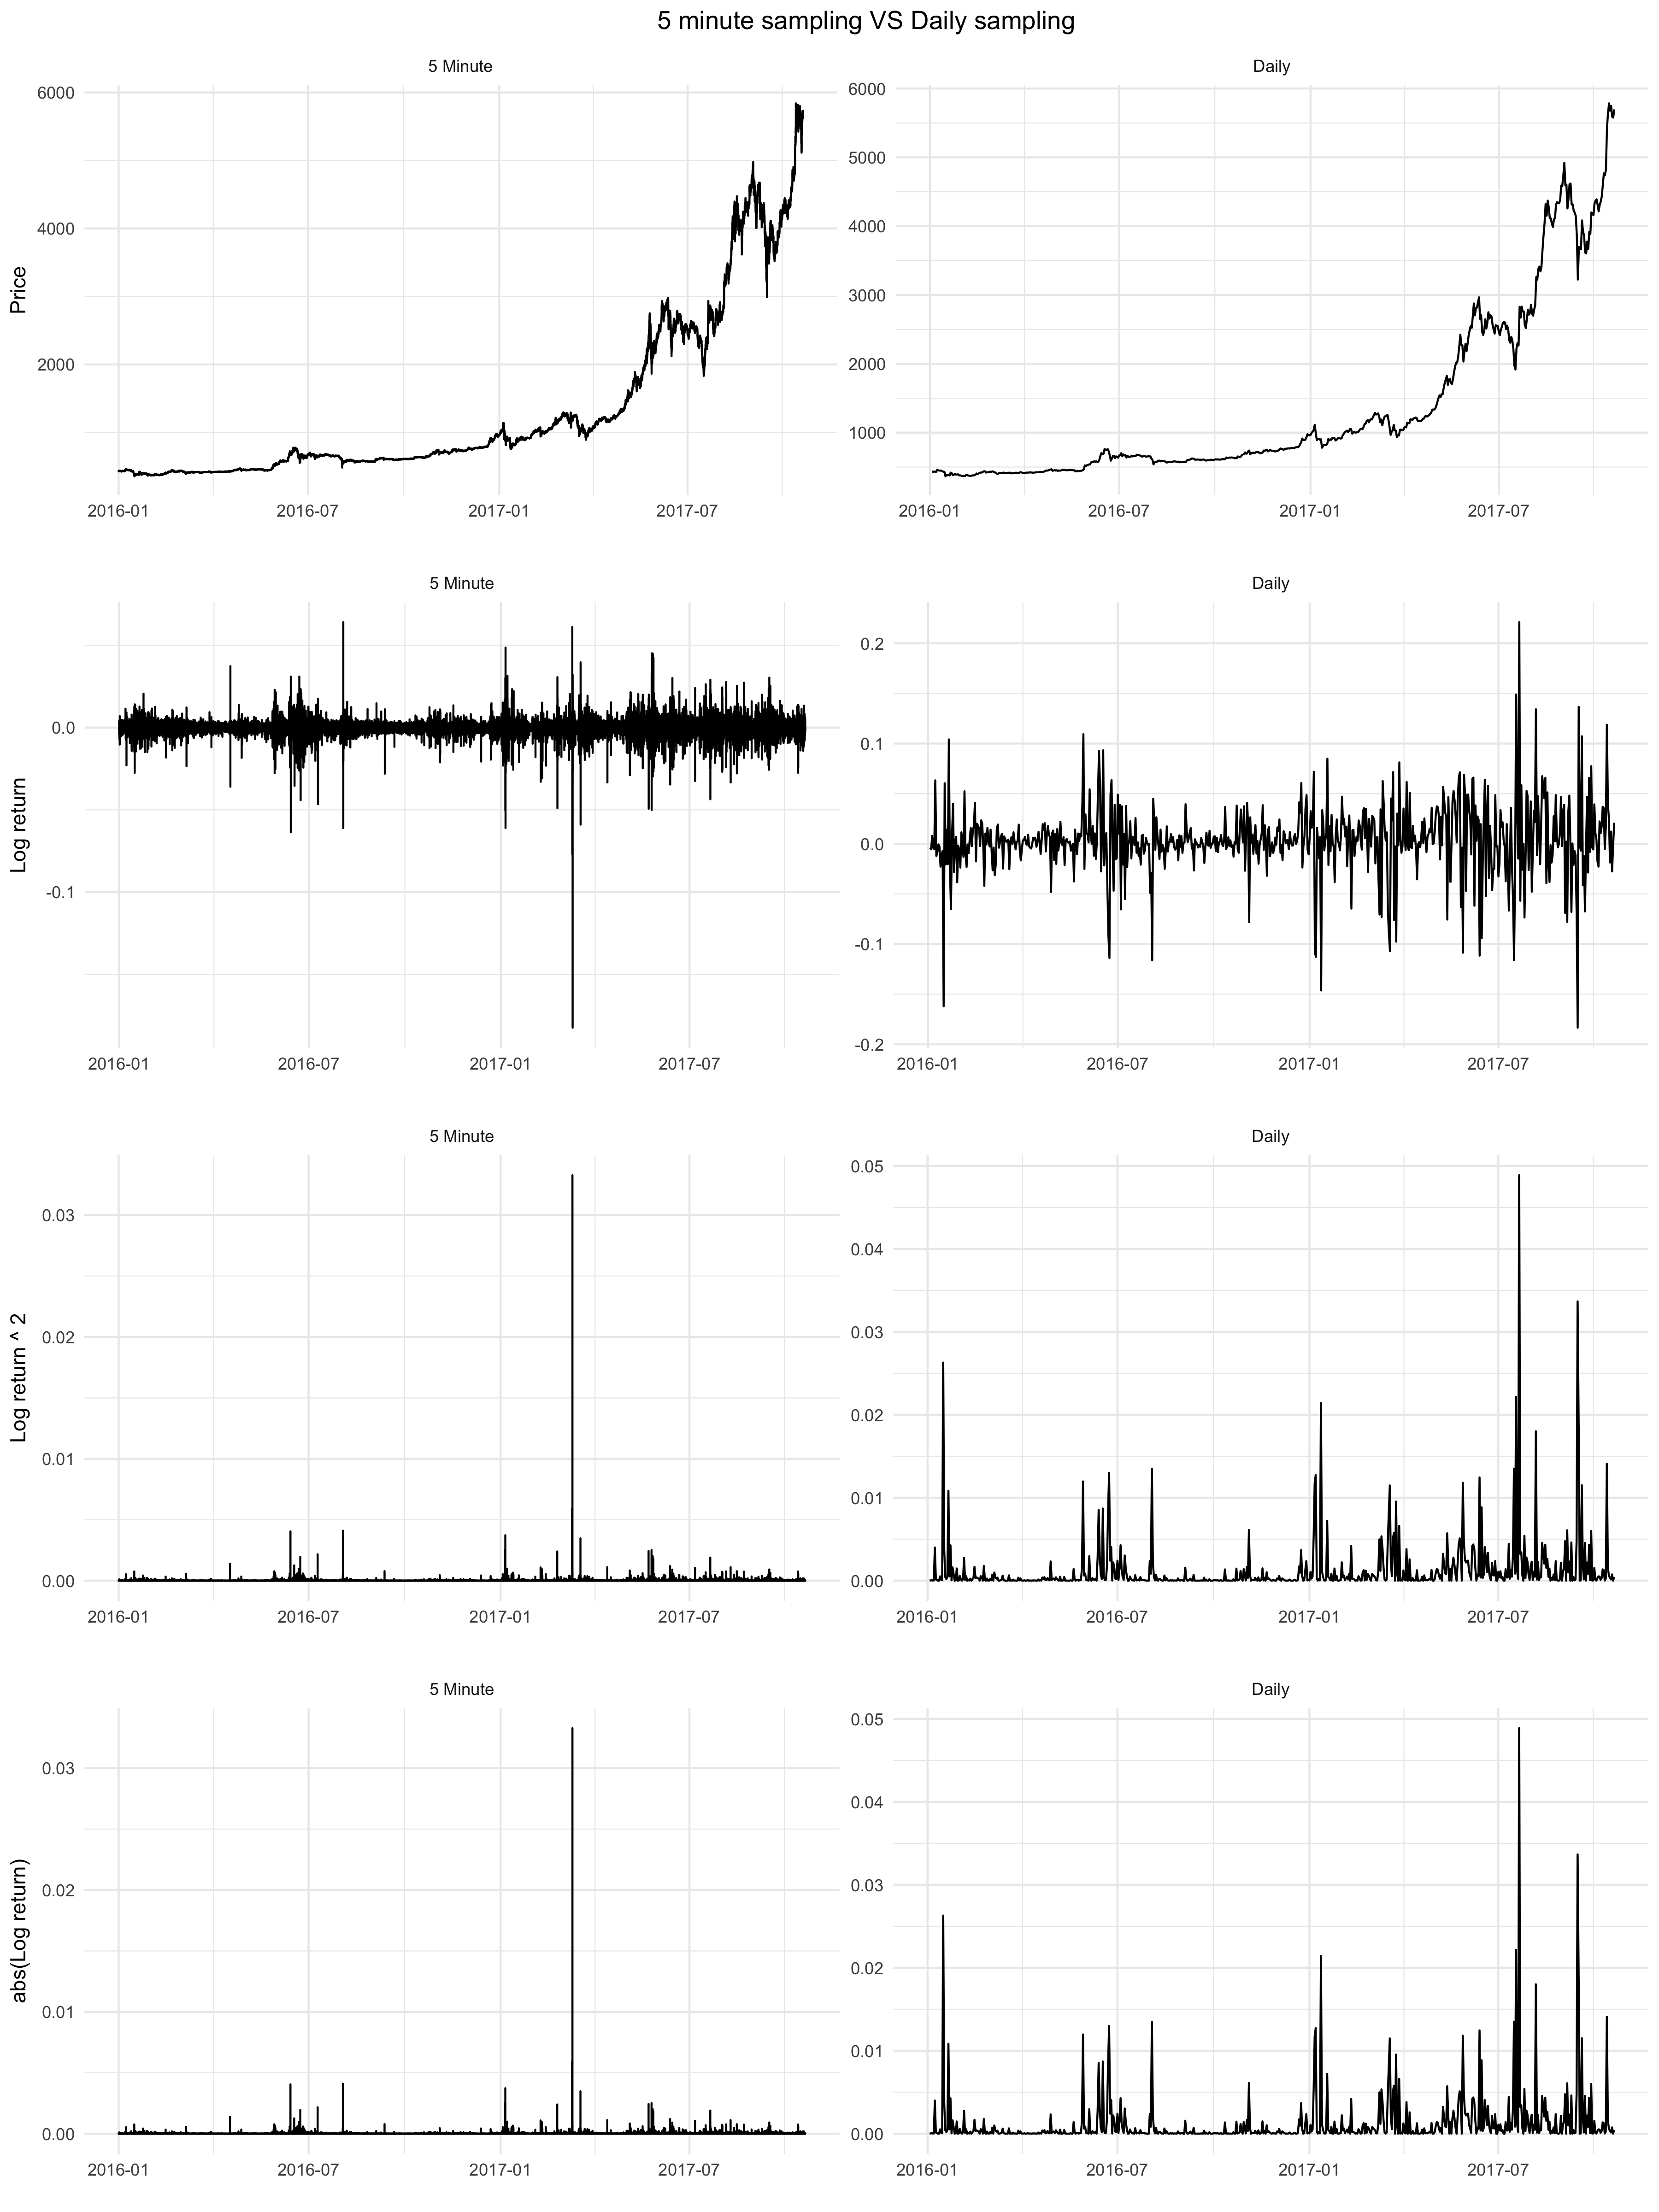
\includegraphics[width=1.00\textwidth, height=8.5in]{../../visualizations/returns} 
  \end{center}
  \caption{Descriptive plots of 5-minute and daily returns}\label{fig}
\end{figure*}

Volatility is modeled using GARCH(1,1) models, fitted at both the
5-minute and daily levels. Two distributions are used for returns,
Normal and Student-t. For simplicity, the mean of the return process is
set to 0. Additionally, after finding it insignificant, the constant in
the GARCH model is set to 0. The resulting model for 5-minute sampling
is,

\begin{equation}
  \begin{aligned}
r_{t_i}         &= \epsilon_{t_i} \\
\epsilon_{t_i}  &= \sigma_{t_i}  z_{t_i} \\
\sigma_{t_i}    &= \alpha \epsilon_{t_{i-1}}  + \beta \sigma_{t_{i-1}}
       \label{eqn:example} 
  \end{aligned}
\end{equation}

with \(z_{t_i}\) represented as either \(z_{t_i} \sim N(0,1)\) or
\(z_{t_i} \sim t_{\nu}\) depending on the underlying distribution. To
differentiate the two distributions, GARCH(1,1)-N and GARCH(1,1)-T will
denote GARCH(1,1) under the Normal and Student-t distributions
respectively. The daily model is defined similarly, with \(t_i\)
replaced by \(d_j\).

\section{In sample estimation
results}\label{in-sample-estimation-results}

The results of the GARCH(1,1) in sample estimations are reported below
in Table 1. Consistent with literature, \(\alpha\) and \(\beta\)
estimates sum to a value close to 1, demonstrating the highly persistent
nature of volatility at both the 5-minute and daily levels. Both
sampling intervals produce a degrees of freedom estimate near 4,
resulting from the heavy tailed nature of the returns. Not shown here
are additional fits from GJR-GARCH models that attempted to capture any
asymmetric properties of the distribution. Interestingly, none of the
asymmetric parameters were statistically significant, suggesting that
Bitcoin does not react more strongly to negative movements.

\begin{table}[h]
\centering\captionsetup{justification=centering,singlelinecheck=off}
\caption{Estimation results of GARCH(1,1) in sample fits under different distributions and at different sampling intervals.}
\begin{tabularx}{0.5\textwidth}{p{0.125\textwidth} p{0.125\textwidth} p{0.125\textwidth} p{0.125\textwidth}}
\multicolumn{1}{!{\color[RGB]{0, 0, 0}\vrule width 0pt}r!{\color[RGB]{0, 0, 0}\vrule width 0.3pt}}{\hspace*{-30pt}\rule{0pt}{\baselineskip+4pt}\raggedleft \textbf{}\rule[-4pt]{0pt}{4pt}\hspace*{4pt}} & 
\multicolumn{1}{c!{\color[RGB]{0, 0, 0}\vrule width 0pt}}{\hspace*{4pt}\rule{0pt}{\baselineskip+4pt}\centering \textbf{ Estimate}\rule[-4pt]{0pt}{4pt}\hspace*{4pt}} & 
\multicolumn{1}{c!{\color[RGB]{0, 0, 0}\vrule width 0pt}}{\hspace*{4pt}\rule{0pt}{\baselineskip+4pt}\centering \textbf{Robust Std Error}\rule[-4pt]{0pt}{4pt}\hspace*{4pt}} & 
\multicolumn{1}{c!{\color[RGB]{0, 0, 0}\vrule width 0pt}}{\hspace*{4pt}\rule{0pt}{\baselineskip+4pt}\centering \textbf{P-value}\rule[-4pt]{0pt}{4pt}\hspace*{4pt}}\tabularnewline[-0.5pt]


\hhline{>{\arrayrulecolor[RGB]{0, 0, 0}\global\arrayrulewidth=0.3pt}->{\arrayrulecolor[RGB]{0, 0, 0}\global\arrayrulewidth=0.3pt}|>{\arrayrulecolor[RGB]{0, 0, 0}\global\arrayrulewidth=0.3pt}->{\arrayrulecolor[RGB]{0, 0, 0}\global\arrayrulewidth=0.3pt}->{\arrayrulecolor[RGB]{0, 0, 0}\global\arrayrulewidth=0.3pt}-}
\arrayrulecolor{black}
\multicolumn{1}{!{\color[RGB]{0, 0, 0}\vrule width 0pt}r!{\color[RGB]{0, 0, 0}\vrule width 0.3pt}}{\hspace*{-30pt}\rule{0pt}{\baselineskip+4pt}\raggedleft \textbf{Normal: 5-min}\rule[-4pt]{0pt}{4pt}\hspace*{4pt}} & 
\multicolumn{1}{c!{\color[RGB]{0, 0, 0}\vrule width 0pt}}{\hspace*{4pt}\rule{0pt}{\baselineskip+4pt}\centering \rule[-4pt]{0pt}{4pt}\hspace*{4pt}} & 
\multicolumn{1}{c!{\color[RGB]{0, 0, 0}\vrule width 0pt}}{\hspace*{4pt}\rule{0pt}{\baselineskip+4pt}\centering \rule[-4pt]{0pt}{4pt}\hspace*{4pt}} & 
\multicolumn{1}{c!{\color[RGB]{0, 0, 0}\vrule width 0pt}}{\hspace*{4pt}\rule{0pt}{\baselineskip+4pt}\centering \rule[-4pt]{0pt}{4pt}\hspace*{4pt}}\tabularnewline[-0.5pt]
\multicolumn{1}{!{\color[RGB]{0, 0, 0}\vrule width 0pt}r!{\color[RGB]{0, 0, 0}\vrule width 0.3pt}}{\hspace*{-30pt}\rule{0pt}{\baselineskip+4pt}\raggedleft $\alpha$\rule[-4pt]{0pt}{4pt}\hspace*{4pt}} & 
\multicolumn{1}{c!{\color[RGB]{0, 0, 0}\vrule width 0pt}}{\hspace*{4pt}\rule{0pt}{\baselineskip+4pt}\centering 0.048\rule[-4pt]{0pt}{4pt}\hspace*{4pt}} & 
\multicolumn{1}{c!{\color[RGB]{0, 0, 0}\vrule width 0pt}}{\hspace*{4pt}\rule{0pt}{\baselineskip+4pt}\centering 0.001\rule[-4pt]{0pt}{4pt}\hspace*{4pt}} & 
\multicolumn{1}{c!{\color[RGB]{0, 0, 0}\vrule width 0pt}}{\hspace*{4pt}\rule{0pt}{\baselineskip+4pt}\centering 0.000\rule[-4pt]{0pt}{4pt}\hspace*{4pt}}\tabularnewline[-0.5pt]
\multicolumn{1}{!{\color[RGB]{0, 0, 0}\vrule width 0pt}r!{\color[RGB]{0, 0, 0}\vrule width 0.3pt}}{\hspace*{-30pt}\rule{0pt}{\baselineskip+4pt}\raggedleft $\beta$\rule[-4pt]{0pt}{4pt}\hspace*{4pt}} & 
\multicolumn{1}{c!{\color[RGB]{0, 0, 0}\vrule width 0pt}}{\hspace*{4pt}\rule{0pt}{\baselineskip+4pt}\centering 0.951\rule[-4pt]{0pt}{4pt}\hspace*{4pt}} & 
\multicolumn{1}{c!{\color[RGB]{0, 0, 0}\vrule width 0pt}}{\hspace*{4pt}\rule{0pt}{\baselineskip+4pt}\centering 0.001\rule[-4pt]{0pt}{4pt}\hspace*{4pt}} & 
\multicolumn{1}{c!{\color[RGB]{0, 0, 0}\vrule width 0pt}}{\hspace*{4pt}\rule{0pt}{\baselineskip+4pt}\centering 0.000\rule[-4pt]{0pt}{4pt}\hspace*{4pt}}\tabularnewline[-0.5pt]


\hhline{>{\arrayrulecolor[RGB]{0, 0, 0}\global\arrayrulewidth=0.3pt}->{\arrayrulecolor[RGB]{0, 0, 0}\global\arrayrulewidth=0.3pt}|>{\arrayrulecolor[RGB]{0, 0, 0}\global\arrayrulewidth=0.3pt}->{\arrayrulecolor[RGB]{0, 0, 0}\global\arrayrulewidth=0.3pt}->{\arrayrulecolor[RGB]{0, 0, 0}\global\arrayrulewidth=0.3pt}-}
\arrayrulecolor{black}
\multicolumn{1}{!{\color[RGB]{0, 0, 0}\vrule width 0pt}r!{\color[RGB]{0, 0, 0}\vrule width 0.3pt}}{\hspace*{-30pt}\rule{0pt}{\baselineskip+4pt}\raggedleft \textbf{Student-t: 5-min}\rule[-4pt]{0pt}{4pt}\hspace*{4pt}} & 
\multicolumn{1}{c!{\color[RGB]{0, 0, 0}\vrule width 0pt}}{\hspace*{4pt}\rule{0pt}{\baselineskip+4pt}\centering \rule[-4pt]{0pt}{4pt}\hspace*{4pt}} & 
\multicolumn{1}{c!{\color[RGB]{0, 0, 0}\vrule width 0pt}}{\hspace*{4pt}\rule{0pt}{\baselineskip+4pt}\centering \rule[-4pt]{0pt}{4pt}\hspace*{4pt}} & 
\multicolumn{1}{c!{\color[RGB]{0, 0, 0}\vrule width 0pt}}{\hspace*{4pt}\rule{0pt}{\baselineskip+4pt}\centering \rule[-4pt]{0pt}{4pt}\hspace*{4pt}}\tabularnewline[-0.5pt]
\multicolumn{1}{!{\color[RGB]{0, 0, 0}\vrule width 0pt}r!{\color[RGB]{0, 0, 0}\vrule width 0.3pt}}{\hspace*{-30pt}\rule{0pt}{\baselineskip+4pt}\raggedleft $\alpha$\rule[-4pt]{0pt}{4pt}\hspace*{4pt}} & 
\multicolumn{1}{c!{\color[RGB]{0, 0, 0}\vrule width 0pt}}{\hspace*{4pt}\rule{0pt}{\baselineskip+4pt}\centering 0.108\rule[-4pt]{0pt}{4pt}\hspace*{4pt}} & 
\multicolumn{1}{c!{\color[RGB]{0, 0, 0}\vrule width 0pt}}{\hspace*{4pt}\rule{0pt}{\baselineskip+4pt}\centering 0.003\rule[-4pt]{0pt}{4pt}\hspace*{4pt}} & 
\multicolumn{1}{c!{\color[RGB]{0, 0, 0}\vrule width 0pt}}{\hspace*{4pt}\rule{0pt}{\baselineskip+4pt}\centering 0.000\rule[-4pt]{0pt}{4pt}\hspace*{4pt}}\tabularnewline[-0.5pt]
\multicolumn{1}{!{\color[RGB]{0, 0, 0}\vrule width 0pt}r!{\color[RGB]{0, 0, 0}\vrule width 0.3pt}}{\hspace*{-30pt}\rule{0pt}{\baselineskip+4pt}\raggedleft $\beta$\rule[-4pt]{0pt}{4pt}\hspace*{4pt}} & 
\multicolumn{1}{c!{\color[RGB]{0, 0, 0}\vrule width 0pt}}{\hspace*{4pt}\rule{0pt}{\baselineskip+4pt}\centering 0.891\rule[-4pt]{0pt}{4pt}\hspace*{4pt}} & 
\multicolumn{1}{c!{\color[RGB]{0, 0, 0}\vrule width 0pt}}{\hspace*{4pt}\rule{0pt}{\baselineskip+4pt}\centering 0.004\rule[-4pt]{0pt}{4pt}\hspace*{4pt}} & 
\multicolumn{1}{c!{\color[RGB]{0, 0, 0}\vrule width 0pt}}{\hspace*{4pt}\rule{0pt}{\baselineskip+4pt}\centering 0.000\rule[-4pt]{0pt}{4pt}\hspace*{4pt}}\tabularnewline[-0.5pt]
\multicolumn{1}{!{\color[RGB]{0, 0, 0}\vrule width 0pt}r!{\color[RGB]{0, 0, 0}\vrule width 0.3pt}}{\hspace*{-30pt}\rule{0pt}{\baselineskip+4pt}\raggedleft $\nu$\rule[-4pt]{0pt}{4pt}\hspace*{4pt}} & 
\multicolumn{1}{c!{\color[RGB]{0, 0, 0}\vrule width 0pt}}{\hspace*{4pt}\rule{0pt}{\baselineskip+4pt}\centering 3.927\rule[-4pt]{0pt}{4pt}\hspace*{4pt}} & 
\multicolumn{1}{c!{\color[RGB]{0, 0, 0}\vrule width 0pt}}{\hspace*{4pt}\rule{0pt}{\baselineskip+4pt}\centering 0.030\rule[-4pt]{0pt}{4pt}\hspace*{4pt}} & 
\multicolumn{1}{c!{\color[RGB]{0, 0, 0}\vrule width 0pt}}{\hspace*{4pt}\rule{0pt}{\baselineskip+4pt}\centering 0.000\rule[-4pt]{0pt}{4pt}\hspace*{4pt}}\tabularnewline[-0.5pt]


\hhline{>{\arrayrulecolor[RGB]{0, 0, 0}\global\arrayrulewidth=0.3pt}->{\arrayrulecolor[RGB]{0, 0, 0}\global\arrayrulewidth=0.3pt}|>{\arrayrulecolor[RGB]{0, 0, 0}\global\arrayrulewidth=0.3pt}->{\arrayrulecolor[RGB]{0, 0, 0}\global\arrayrulewidth=0.3pt}->{\arrayrulecolor[RGB]{0, 0, 0}\global\arrayrulewidth=0.3pt}-}
\arrayrulecolor{black}
\multicolumn{1}{!{\color[RGB]{0, 0, 0}\vrule width 0pt}r!{\color[RGB]{0, 0, 0}\vrule width 0.3pt}}{\hspace*{-30pt}\rule{0pt}{\baselineskip+4pt}\raggedleft \textbf{Normal: daily}\rule[-4pt]{0pt}{4pt}\hspace*{4pt}} & 
\multicolumn{1}{c!{\color[RGB]{0, 0, 0}\vrule width 0pt}}{\hspace*{4pt}\rule{0pt}{\baselineskip+4pt}\centering \rule[-4pt]{0pt}{4pt}\hspace*{4pt}} & 
\multicolumn{1}{c!{\color[RGB]{0, 0, 0}\vrule width 0pt}}{\hspace*{4pt}\rule{0pt}{\baselineskip+4pt}\centering \rule[-4pt]{0pt}{4pt}\hspace*{4pt}} & 
\multicolumn{1}{c!{\color[RGB]{0, 0, 0}\vrule width 0pt}}{\hspace*{4pt}\rule{0pt}{\baselineskip+4pt}\centering \rule[-4pt]{0pt}{4pt}\hspace*{4pt}}\tabularnewline[-0.5pt]
\multicolumn{1}{!{\color[RGB]{0, 0, 0}\vrule width 0pt}r!{\color[RGB]{0, 0, 0}\vrule width 0.3pt}}{\hspace*{-30pt}\rule{0pt}{\baselineskip+4pt}\raggedleft $\alpha$\rule[-4pt]{0pt}{4pt}\hspace*{4pt}} & 
\multicolumn{1}{c!{\color[RGB]{0, 0, 0}\vrule width 0pt}}{\hspace*{4pt}\rule{0pt}{\baselineskip+4pt}\centering 0.086\rule[-4pt]{0pt}{4pt}\hspace*{4pt}} & 
\multicolumn{1}{c!{\color[RGB]{0, 0, 0}\vrule width 0pt}}{\hspace*{4pt}\rule{0pt}{\baselineskip+4pt}\centering 0.027\rule[-4pt]{0pt}{4pt}\hspace*{4pt}} & 
\multicolumn{1}{c!{\color[RGB]{0, 0, 0}\vrule width 0pt}}{\hspace*{4pt}\rule{0pt}{\baselineskip+4pt}\centering 0.001\rule[-4pt]{0pt}{4pt}\hspace*{4pt}}\tabularnewline[-0.5pt]
\multicolumn{1}{!{\color[RGB]{0, 0, 0}\vrule width 0pt}r!{\color[RGB]{0, 0, 0}\vrule width 0.3pt}}{\hspace*{-30pt}\rule{0pt}{\baselineskip+4pt}\raggedleft $\beta$\rule[-4pt]{0pt}{4pt}\hspace*{4pt}} & 
\multicolumn{1}{c!{\color[RGB]{0, 0, 0}\vrule width 0pt}}{\hspace*{4pt}\rule{0pt}{\baselineskip+4pt}\centering 0.913\rule[-4pt]{0pt}{4pt}\hspace*{4pt}} & 
\multicolumn{1}{c!{\color[RGB]{0, 0, 0}\vrule width 0pt}}{\hspace*{4pt}\rule{0pt}{\baselineskip+4pt}\centering 0.030\rule[-4pt]{0pt}{4pt}\hspace*{4pt}} & 
\multicolumn{1}{c!{\color[RGB]{0, 0, 0}\vrule width 0pt}}{\hspace*{4pt}\rule{0pt}{\baselineskip+4pt}\centering 0.000\rule[-4pt]{0pt}{4pt}\hspace*{4pt}}\tabularnewline[-0.5pt]


\hhline{>{\arrayrulecolor[RGB]{0, 0, 0}\global\arrayrulewidth=0.3pt}->{\arrayrulecolor[RGB]{0, 0, 0}\global\arrayrulewidth=0.3pt}|>{\arrayrulecolor[RGB]{0, 0, 0}\global\arrayrulewidth=0.3pt}->{\arrayrulecolor[RGB]{0, 0, 0}\global\arrayrulewidth=0.3pt}->{\arrayrulecolor[RGB]{0, 0, 0}\global\arrayrulewidth=0.3pt}-}
\arrayrulecolor{black}
\multicolumn{1}{!{\color[RGB]{0, 0, 0}\vrule width 0pt}r!{\color[RGB]{0, 0, 0}\vrule width 0.3pt}}{\hspace*{-30pt}\rule{0pt}{\baselineskip+4pt}\raggedleft \textbf{Student-t: daily}\rule[-4pt]{0pt}{4pt}\hspace*{4pt}} & 
\multicolumn{1}{c!{\color[RGB]{0, 0, 0}\vrule width 0pt}}{\hspace*{4pt}\rule{0pt}{\baselineskip+4pt}\centering \rule[-4pt]{0pt}{4pt}\hspace*{4pt}} & 
\multicolumn{1}{c!{\color[RGB]{0, 0, 0}\vrule width 0pt}}{\hspace*{4pt}\rule{0pt}{\baselineskip+4pt}\centering \rule[-4pt]{0pt}{4pt}\hspace*{4pt}} & 
\multicolumn{1}{c!{\color[RGB]{0, 0, 0}\vrule width 0pt}}{\hspace*{4pt}\rule{0pt}{\baselineskip+4pt}\centering \rule[-4pt]{0pt}{4pt}\hspace*{4pt}}\tabularnewline[-0.5pt]
\multicolumn{1}{!{\color[RGB]{0, 0, 0}\vrule width 0pt}r!{\color[RGB]{0, 0, 0}\vrule width 0.3pt}}{\hspace*{-30pt}\rule{0pt}{\baselineskip+4pt}\raggedleft $\alpha$\rule[-4pt]{0pt}{4pt}\hspace*{4pt}} & 
\multicolumn{1}{c!{\color[RGB]{0, 0, 0}\vrule width 0pt}}{\hspace*{4pt}\rule{0pt}{\baselineskip+4pt}\centering 0.142\rule[-4pt]{0pt}{4pt}\hspace*{4pt}} & 
\multicolumn{1}{c!{\color[RGB]{0, 0, 0}\vrule width 0pt}}{\hspace*{4pt}\rule{0pt}{\baselineskip+4pt}\centering 0.027\rule[-4pt]{0pt}{4pt}\hspace*{4pt}} & 
\multicolumn{1}{c!{\color[RGB]{0, 0, 0}\vrule width 0pt}}{\hspace*{4pt}\rule{0pt}{\baselineskip+4pt}\centering 0.000\rule[-4pt]{0pt}{4pt}\hspace*{4pt}}\tabularnewline[-0.5pt]
\multicolumn{1}{!{\color[RGB]{0, 0, 0}\vrule width 0pt}r!{\color[RGB]{0, 0, 0}\vrule width 0.3pt}}{\hspace*{-30pt}\rule{0pt}{\baselineskip+4pt}\raggedleft $\beta$\rule[-4pt]{0pt}{4pt}\hspace*{4pt}} & 
\multicolumn{1}{c!{\color[RGB]{0, 0, 0}\vrule width 0pt}}{\hspace*{4pt}\rule{0pt}{\baselineskip+4pt}\centering 0.857\rule[-4pt]{0pt}{4pt}\hspace*{4pt}} & 
\multicolumn{1}{c!{\color[RGB]{0, 0, 0}\vrule width 0pt}}{\hspace*{4pt}\rule{0pt}{\baselineskip+4pt}\centering 0.031\rule[-4pt]{0pt}{4pt}\hspace*{4pt}} & 
\multicolumn{1}{c!{\color[RGB]{0, 0, 0}\vrule width 0pt}}{\hspace*{4pt}\rule{0pt}{\baselineskip+4pt}\centering 0.000\rule[-4pt]{0pt}{4pt}\hspace*{4pt}}\tabularnewline[-0.5pt]
\multicolumn{1}{!{\color[RGB]{0, 0, 0}\vrule width 0pt}r!{\color[RGB]{0, 0, 0}\vrule width 0.3pt}}{\hspace*{-30pt}\rule{0pt}{\baselineskip+4pt}\raggedleft $\nu$\rule[-4pt]{0pt}{4pt}\hspace*{4pt}} & 
\multicolumn{1}{c!{\color[RGB]{0, 0, 0}\vrule width 0pt}}{\hspace*{4pt}\rule{0pt}{\baselineskip+4pt}\centering 3.619\rule[-4pt]{0pt}{4pt}\hspace*{4pt}} & 
\multicolumn{1}{c!{\color[RGB]{0, 0, 0}\vrule width 0pt}}{\hspace*{4pt}\rule{0pt}{\baselineskip+4pt}\centering 0.318\rule[-4pt]{0pt}{4pt}\hspace*{4pt}} & 
\multicolumn{1}{c!{\color[RGB]{0, 0, 0}\vrule width 0pt}}{\hspace*{4pt}\rule{0pt}{\baselineskip+4pt}\centering 0.000\rule[-4pt]{0pt}{4pt}\hspace*{4pt}}\tabularnewline[-0.5pt]
\end{tabularx}

\end{table}

\section{Volatility forecasting and realized
variance}\label{volatility-forecasting-and-realized-variance}

The forecasting methods used can be broken down into two sections: the
procedure used for including new information in the forecasts, and the
performance measure used to validate against.

\subsection{Forecasting methodology}\label{forecasting-methodology}

For daily sampling, the forecasting procedure is as follows:

\begin{enumerate}
\def\labelenumi{\arabic{enumi})}
\tightlist
\item
  An initial GARCH(1,1) model is fit using the first 546 daily returns.
\item
  A 1-step ahead forecast of the next day's variance is generated,
  denoted \(\hat{h}_{d_{j+1}}\).
\item
  Using a moving window, the oldest day's return is dropped, the newest
  day's return is included, and the model is refit.
\item
  Steps 2 and 3 are repeated to generate 111 daily forecasts of
  variance.
\end{enumerate}

For 5-minute sampling, the forecasting procedure is slightly more
complicated to avoid any look ahead bias. The procedure is:

\begin{enumerate}
\def\labelenumi{\arabic{enumi})}
\tightlist
\item
  An initial GARCH(1,1) model is fit using the first 157535 5-minute
  returns. This ends the fit on 2017-06-30 23:55:00, the end of that
  day.
\item
  The next day's worth of 5-minute variance forecasts are generated
  recursively. This results in 288 5-minute forecasts for the next day
  (24 hours x 60 minutes / 5 minutes).
\item
  Those 5-minute forecasts are summed to generate a forecast of variance
  for that day, denoted
  \(\hat{H}_{d_{j+1}} = \sum_{i = 1}^{288} \hat{h}_{t_{i + 288(j+1)}}\).
  The notation of \(288(j+1)\) is used to ensure that the correct day's
  worth of 5-minute variance forecasts are summed.
\item
  Using a moving window, the oldest 288 5-minute returns are dropped,
  the newest 288 5-minute returns are included, and the model is refit.
  This effectively shifts the model 1 day forward.
\item
  Steps 2-4 are repeated to generate 111 daily forecasts of variance.
\end{enumerate}

Ideally, the aggregation approach allows the model to be more flexible,
and take into account a finer level of detail. These approaches were
repeated for both Normal and Student-t distributions.

To generate n-step ahead forecasts under the GARCH(1,1) model, the
following recursive formula was used:

\begin{equation}
  \begin{aligned}
\hat{h}_{t+n} = (\alpha + \beta)^{n-1} \hat{h}_{t+1}
       \label{eqn:forecast} 
  \end{aligned}
\end{equation}

\subsection{Realized variance}\label{realized-variance}

Equally as important as the forecast methodology is the proxy of
variance that one measures performance against. Because volatility is
unobservable, some estimate of the true volatility is required to
calculate any kind of performance measure. A common measure of
forecasting performance for daily variance is to use that day's squared
return, \(r_{d_{j+1}}^2\). However, as noted by Bollershev, while this
is a consistent estimator of conditional variance, it is incredibly
noisy, \cite{Garch}. Bollershev proposes the use of intraday information
to estimate the daily variance. The technique, termed \emph{realized
variance}, is adapted here as the sum of squared returns for the 288
5-minute returns in each day. Formally:

\[ RV_{d_{j+1}} = \sum_{i = 1}^{288} r_{t_{i + 288(j+1)}}^2 \]

Both the daily squared return and the realized variance will be used to
generate performance metrics for the models, and their uses as
benchmarks will be compared.

Figure 2 demonstrates the difference between the proxies of realized
variance and the squared daily return. Squared return is incredibly
noisy in comparison to realized variance, especially in periods of
higher volatility, where the estimate can spike to unrealistically high
amounts.

\begin{figure*}
  \begin{center}
    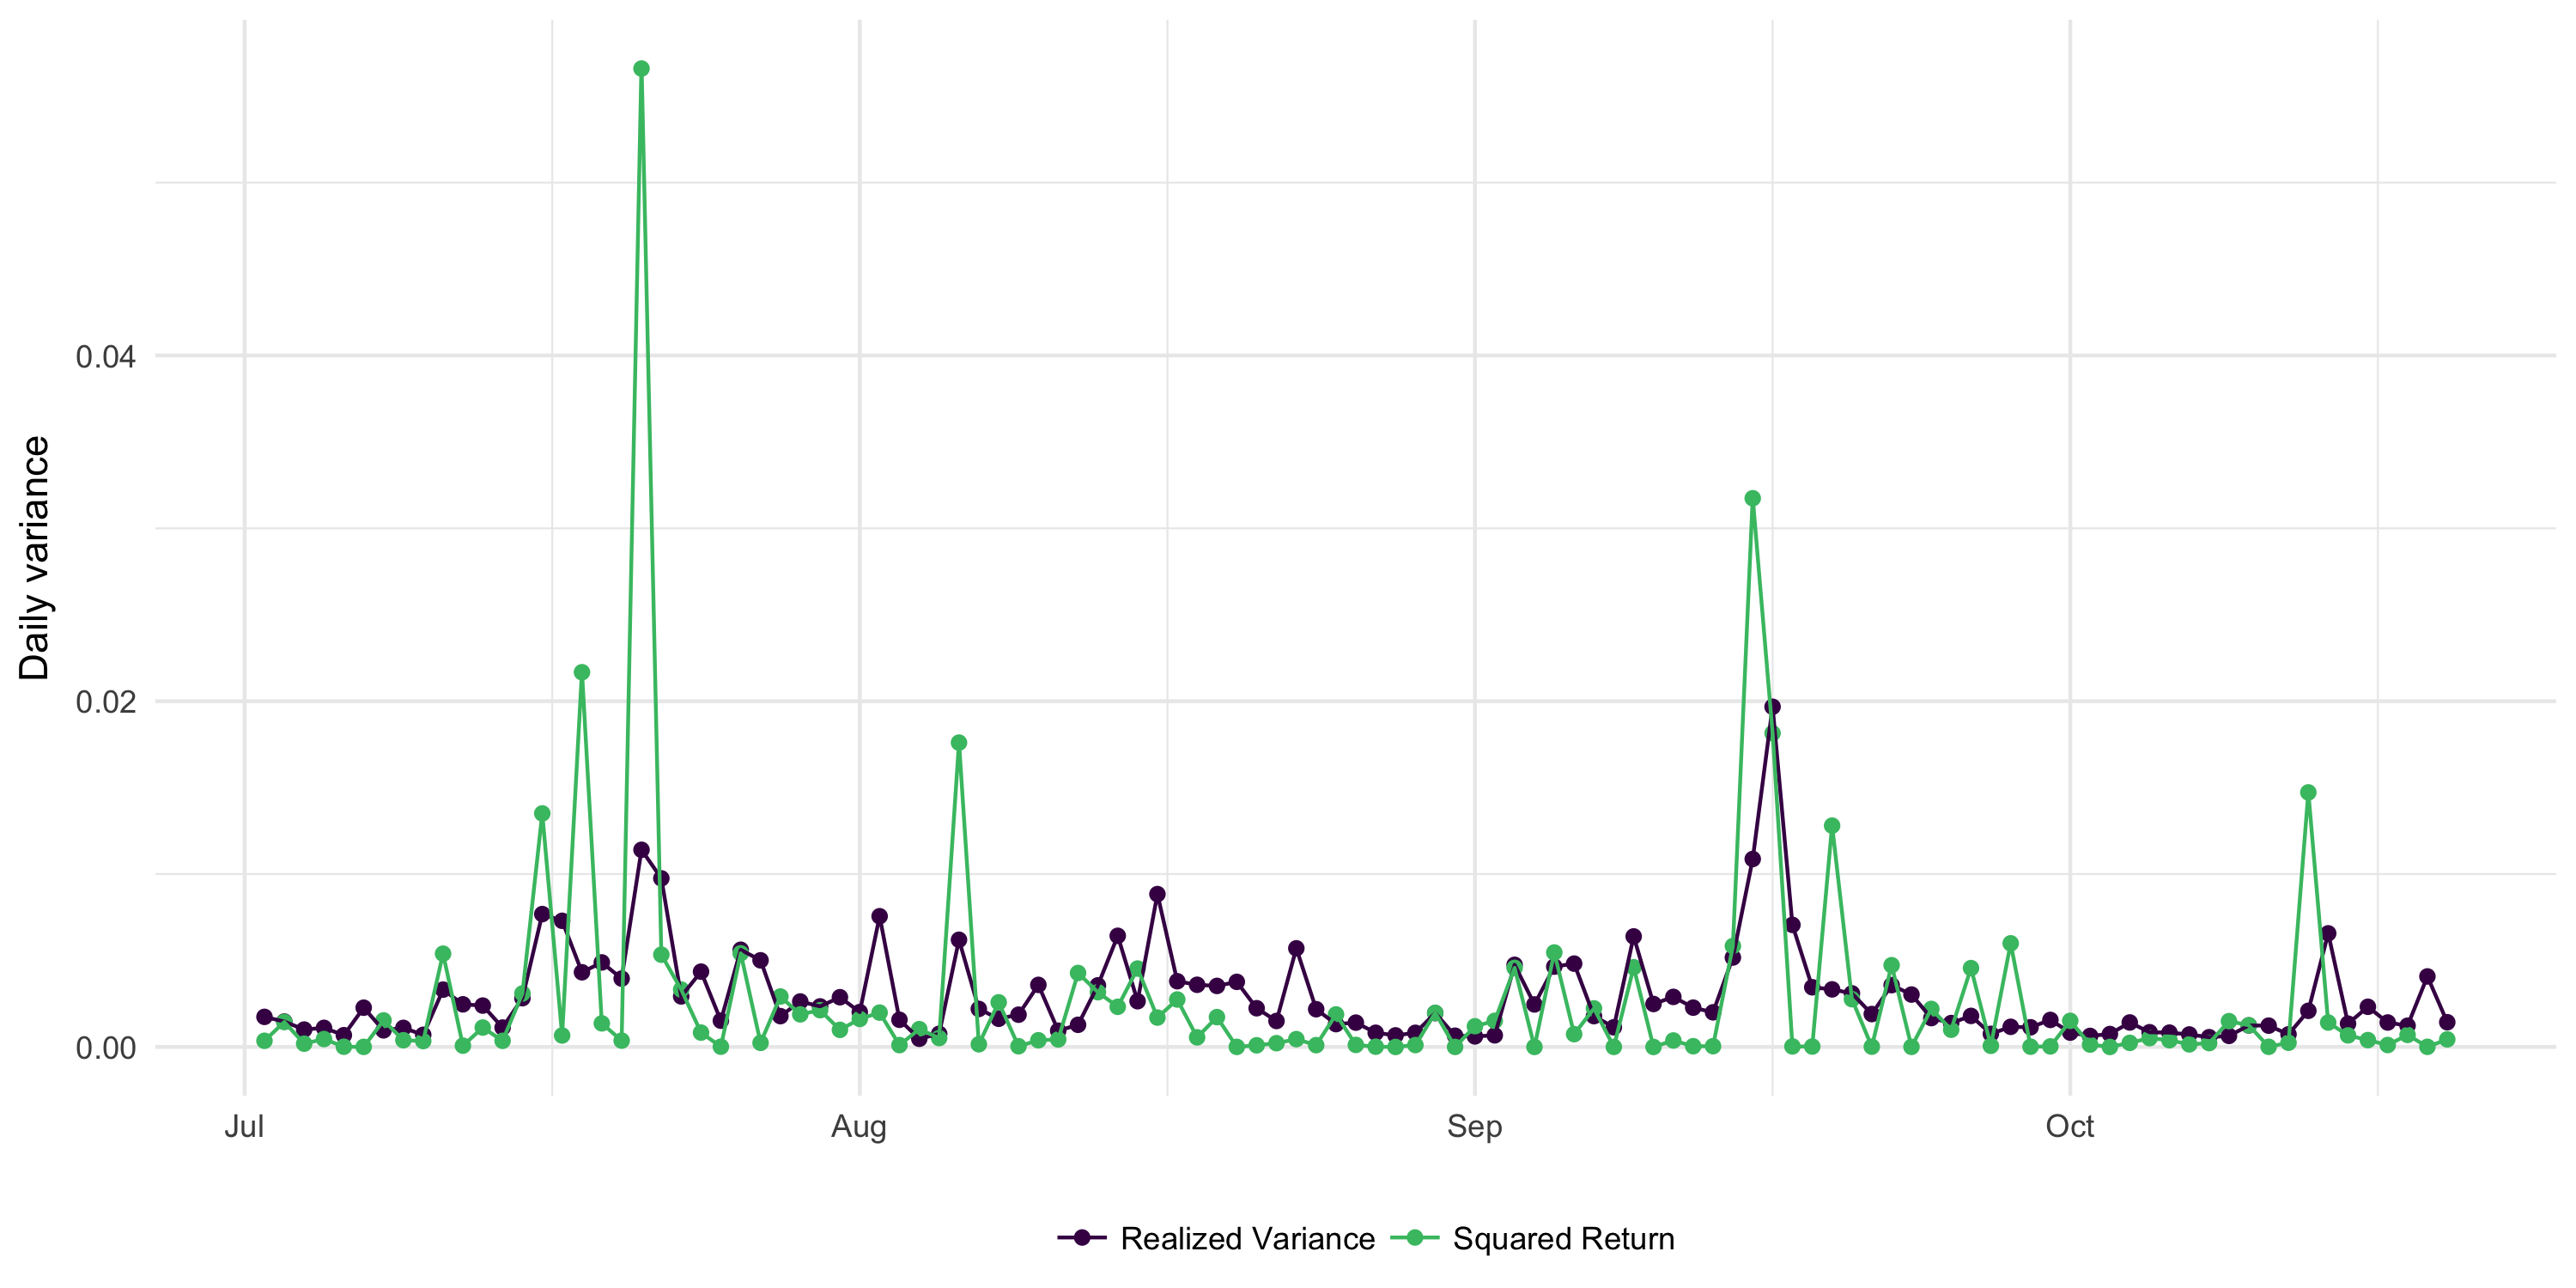
\includegraphics[width=1.00\textwidth]{../../visualizations/compare_proxies} 
  \end{center}
  \caption{Realized variance VS Squared return in the out of sample period. Squared return is very noisy, and not the best estimator to benchmark performance against.}\label{fig}
\end{figure*}

\section{Forecasting results}\label{forecasting-results}

The plot in Figure 3 shows the out of sample forecasting performance of
the GARCH(1,1)-N models in comparision to the realized variance. The
daily forecasts generated from aggregated 5-minute forecasts have more
flexibility to adapt quickly to the movements in the level of variance
compared to the GARCH(1,1)-N model fit to daily data, especially in
transition periods from high to low volatility.

The extreme forecast from the aggregation model resulting in variance
above 0.04 in mid July is of cause for concern, and discussion of this
is addressed in the next section.

\begin{figure*}
  \begin{center}
    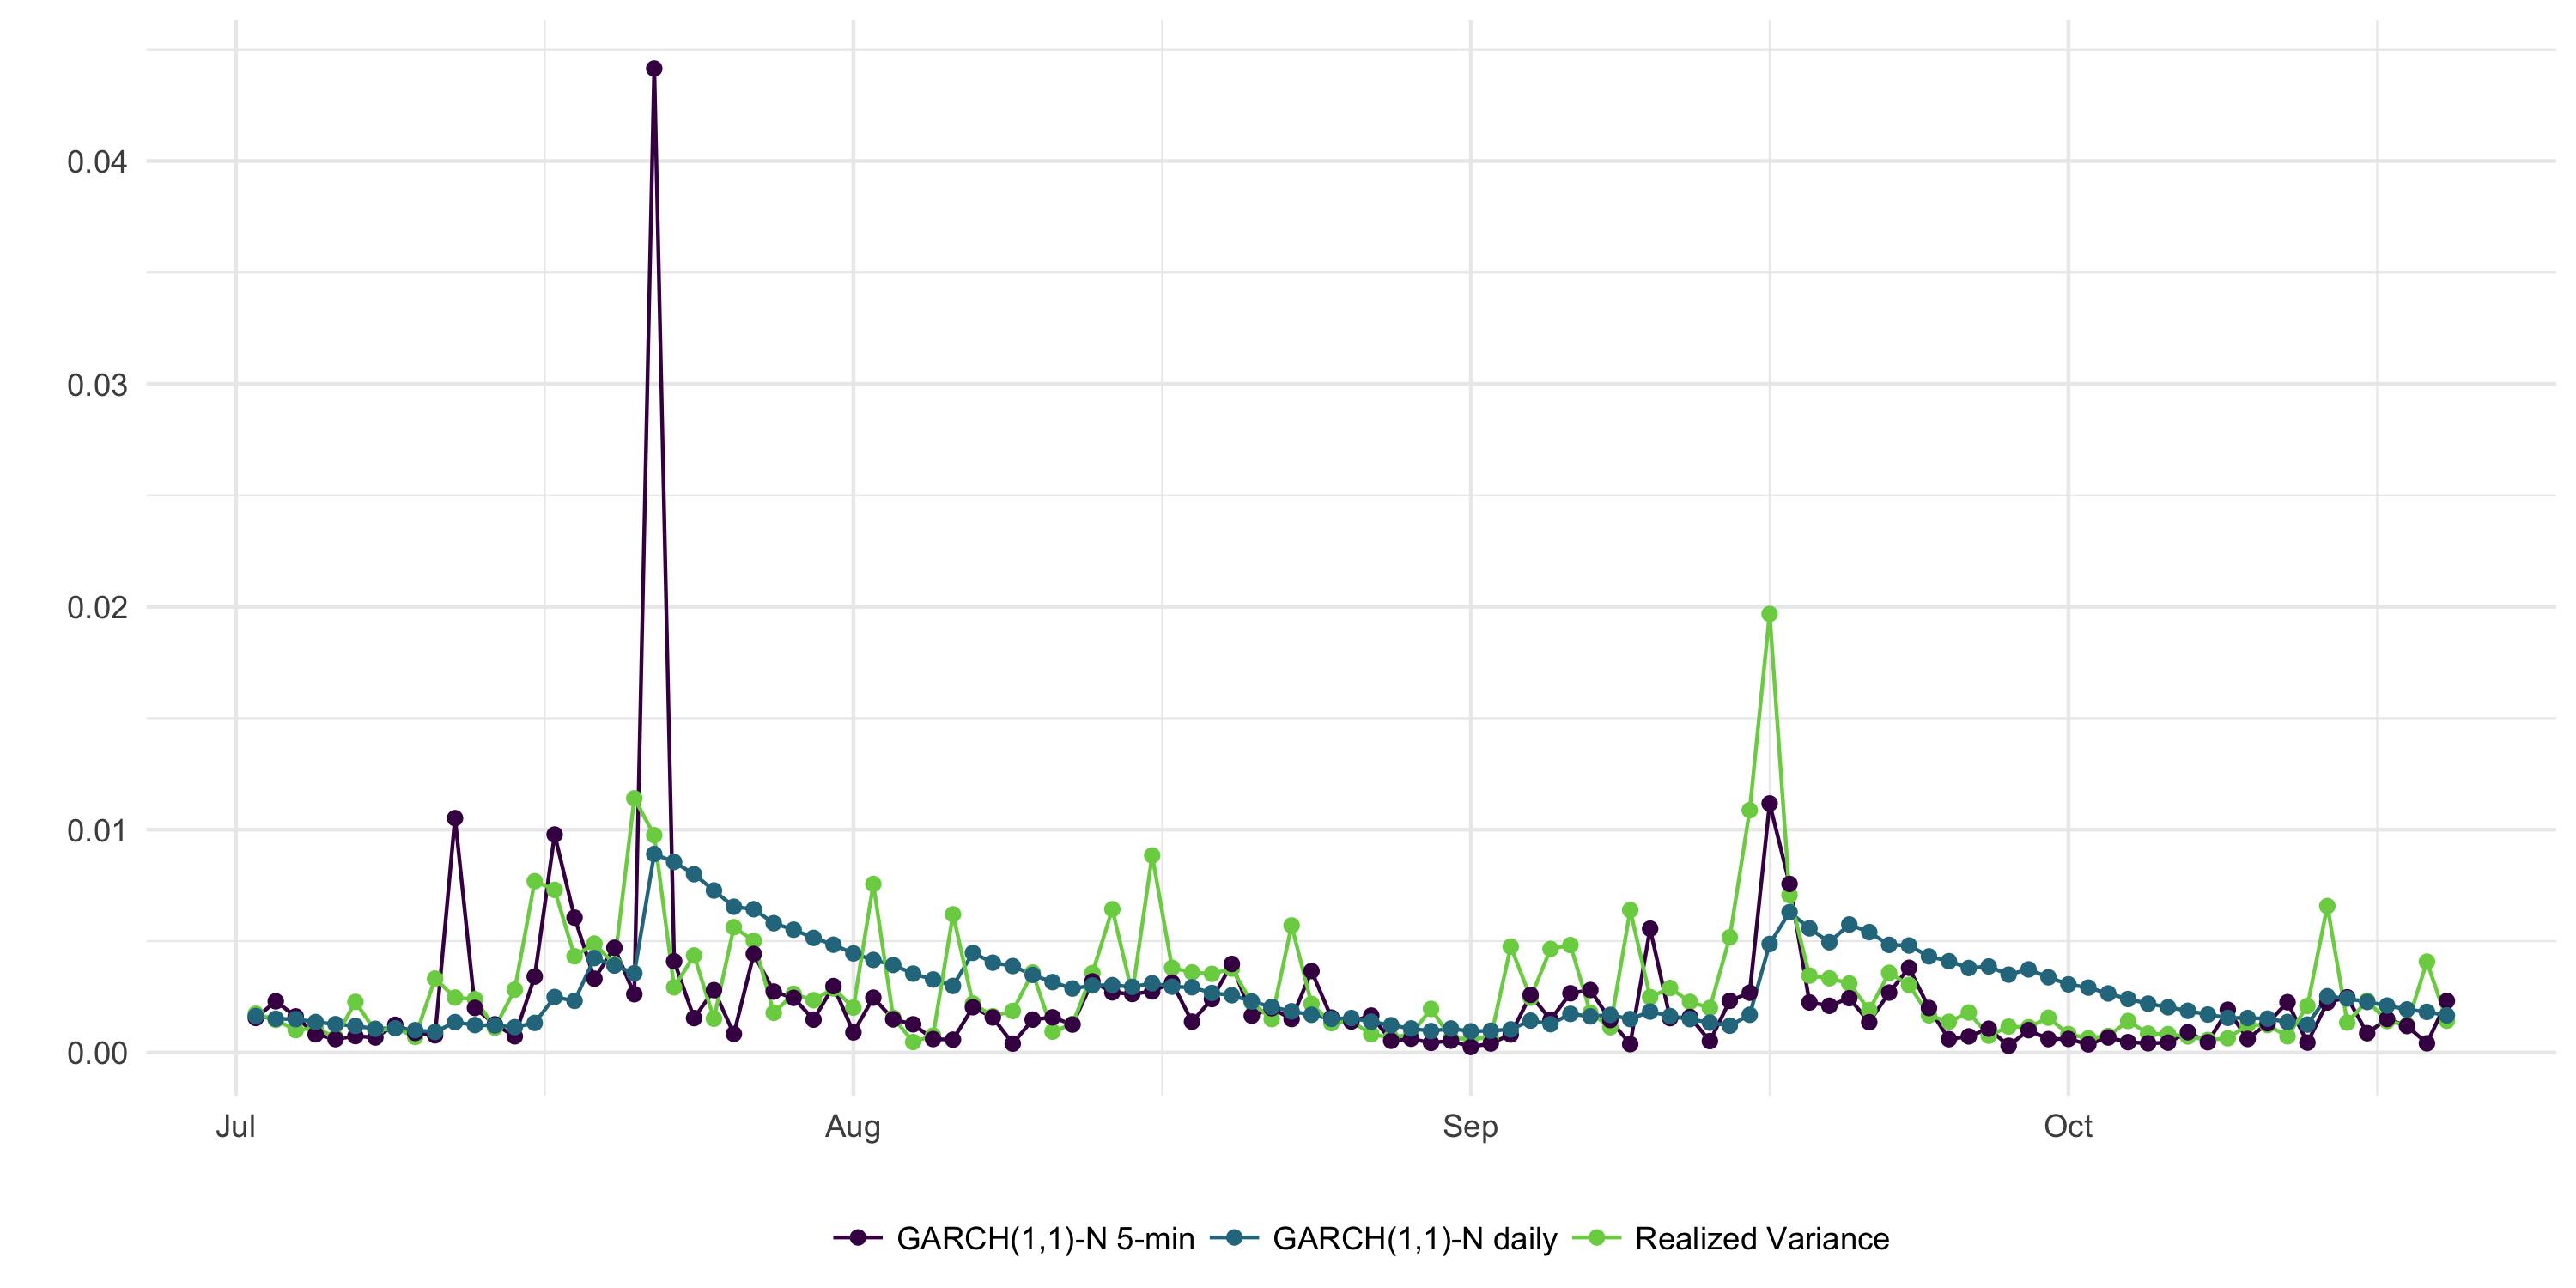
\includegraphics[width=1.00\textwidth]{../../visualizations/compare_normal_forecasts} 
  \end{center}
  \caption{Out of sample performance of GARCH(1,1) models under the Normal distribution. Daily forecasts of variance from aggregated 5-minute forecasts appear to be more flexible in adapting quickly to changes in the overall level of variance, especially in transition periods from high to low variance like mid September.}\label{fig}
\end{figure*}

Figure 4 compares the Normal and Student-t forecasts for the 5-minute
aggregation technique. Student-t forecasts tend to be higher in periods
of high volatility, and slightly lower in periods of lower volatility,
but overall they follow a similar track.

\begin{figure*}
  \begin{center}
    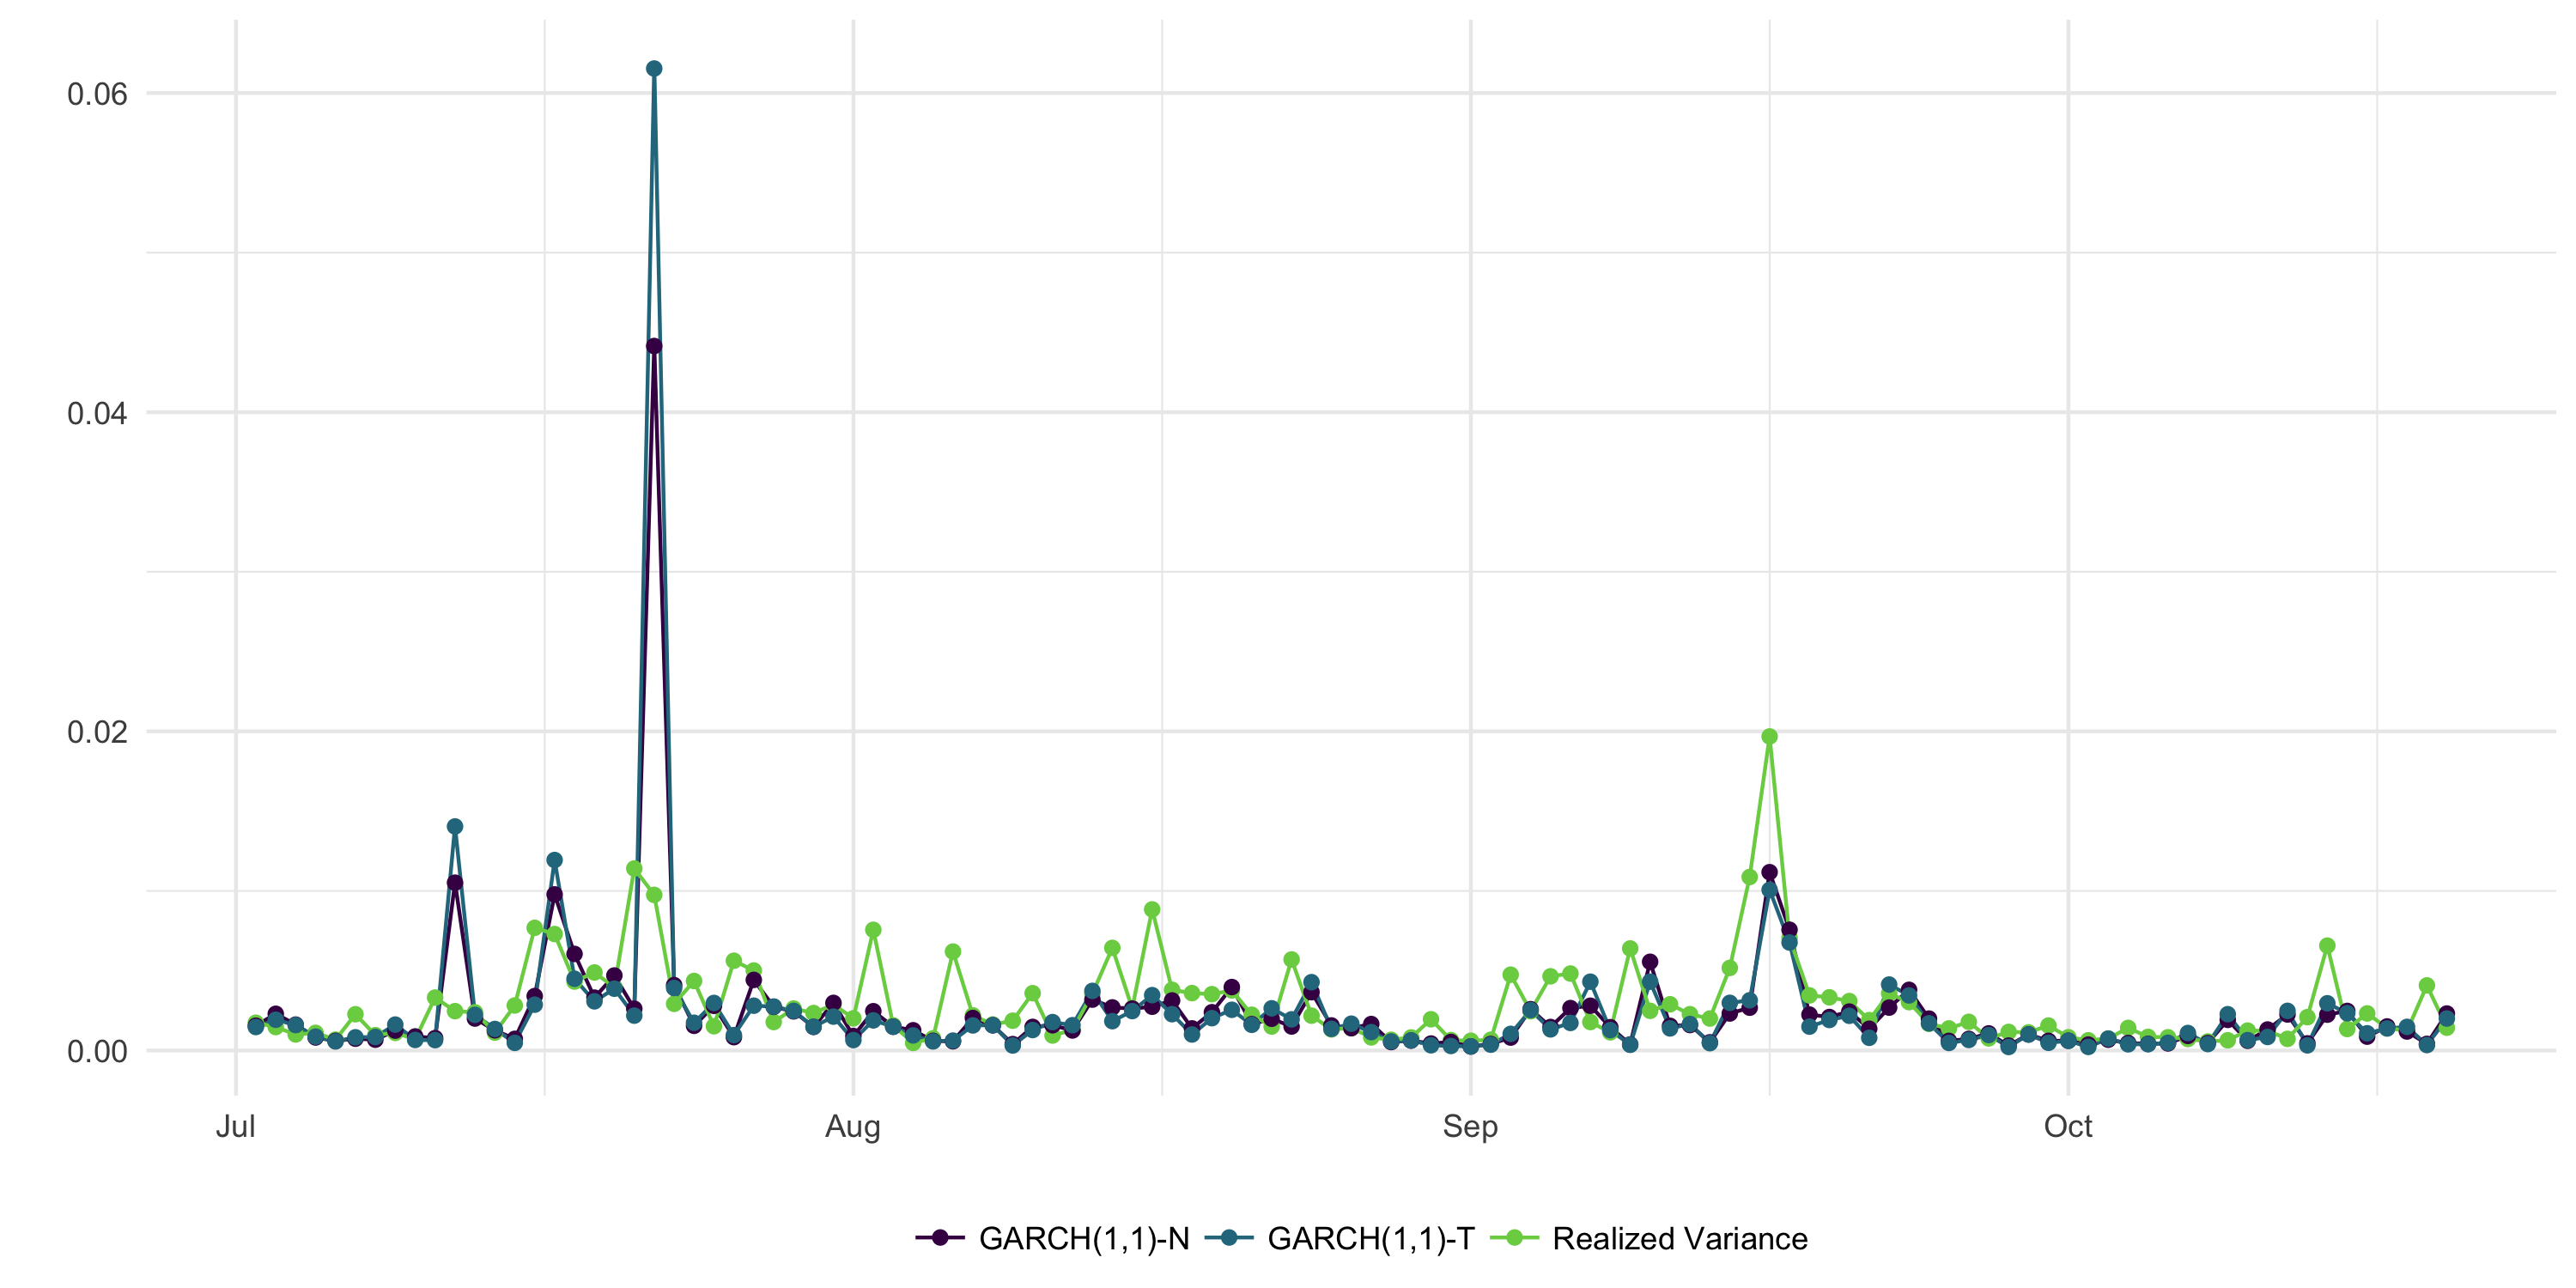
\includegraphics[width=1.00\textwidth]{../../visualizations/compare_normal_vs_student_forecasts} 
  \end{center}
  \caption{Out of sample performance of Normal VS Student-t GARCH(1,1) models
  using the 5-minute aggregation technique. Student-t forecasts tend to swing
  more wildly, but overall there is not much difference.}\label{fig}
\end{figure*}

Table 2 displays a number of performance metrics from the GARCH(1,1)
models under the Normal distribution. For brevity, Student-t results are
not included as they are not very different from Normal. Included
metrics are Mean Absolute Percent Error (MAPE), Root Mean Squared Error
(RMSE), and the intercept, slope and \(R^2\) from Minzer-Zarnowitz (MZ)
regression of the corresponding proxy on the forecasts. For all metrics,
the realized variance proxy implied the models forecasted better than
when compared against the squared daily return proxy.

The first two columns correspond to the 5-minute aggregation method of
daily forecasts, and the forecasts from daily models respectively. While
the MAPE of the 5-minute method is lower than for daily, the RMSE is
much higher. This is a direct result of the incredibly large forecast
above 0.04 from the 5-minute method that can be seen in Figure 3. Column
3 contains the metrics calculated again for the 5-minute method, but
with the removal of that one large forecast. After removing that single
point, the RMSE drops below the daily method, the MZ slope coefficient
jumps up to a value much closer to 1, and the MZ \(R^2\) increases
significantly. This finding prompted a further analysis to attempt to
understand the outlier, outlined in the next section.

\begin{table}[h]
\centering\captionsetup{justification=centering,singlelinecheck=off}
\caption{Out of sample performance of GARCH(1,1) Normal models. MAPE for 5-min is lower than for daily. Across the board, using RV as a proxy over $r^2$ gives more accurate results. Removing the 1 extreme forecast from the 5-min method results in a much higher MZ $R^2$, and a MZ slope much closer to 1.}
\begin{tabularx}{0.5\textwidth}{p{0.125\textwidth} p{0.125\textwidth} p{0.125\textwidth} p{0.125\textwidth}}
\multicolumn{1}{!{\color[RGB]{0, 0, 0}\vrule width 0pt}r!{\color[RGB]{0, 0, 0}\vrule width 0.3pt}}{\hspace*{-40pt}\rule{0pt}{\baselineskip+10pt}\raggedleft \textbf{}\rule[-10pt]{0pt}{10pt}\hspace*{10pt}} & 
\multicolumn{1}{c!{\color[RGB]{0, 0, 0}\vrule width 0pt}}{\hspace*{10pt}\rule{0pt}{\baselineskip+10pt}\centering \textbf{5-Min}\rule[-10pt]{0pt}{10pt}\hspace*{10pt}} & 
\multicolumn{1}{c!{\color[RGB]{0, 0, 0}\vrule width 0pt}}{\hspace*{10pt}\rule{0pt}{\baselineskip+10pt}\centering \textbf{Daily}\rule[-10pt]{0pt}{10pt}\hspace*{10pt}} & 
\multicolumn{1}{c!{\color[RGB]{0, 0, 0}\vrule width 0pt}}{\hspace*{10pt}\rule{0pt}{\baselineskip+10pt}\centering \textbf{5-Min No Outlier}\rule[-10pt]{0pt}{10pt}\hspace*{10pt}}\tabularnewline[-0.5pt]


\hhline{>{\arrayrulecolor[RGB]{0, 0, 0}\global\arrayrulewidth=0.3pt}->{\arrayrulecolor[RGB]{0, 0, 0}\global\arrayrulewidth=0.3pt}|>{\arrayrulecolor[RGB]{0, 0, 0}\global\arrayrulewidth=0.3pt}->{\arrayrulecolor[RGB]{0, 0, 0}\global\arrayrulewidth=0.3pt}->{\arrayrulecolor[RGB]{0, 0, 0}\global\arrayrulewidth=0.3pt}-}
\arrayrulecolor{black}
\multicolumn{1}{!{\color[RGB]{0, 0, 0}\vrule width 0pt}r!{\color[RGB]{0, 0, 0}\vrule width 0.3pt}}{\hspace*{-40pt}\rule{0pt}{\baselineskip+10pt}\raggedleft \textbf{Proxy: RV}\rule[-10pt]{0pt}{10pt}\hspace*{10pt}} & 
\multicolumn{1}{c!{\color[RGB]{0, 0, 0}\vrule width 0pt}}{\hspace*{10pt}\rule{0pt}{\baselineskip+10pt}\centering \rule[-10pt]{0pt}{10pt}\hspace*{10pt}} & 
\multicolumn{1}{c!{\color[RGB]{0, 0, 0}\vrule width 0pt}}{\hspace*{10pt}\rule{0pt}{\baselineskip+10pt}\centering \rule[-10pt]{0pt}{10pt}\hspace*{10pt}} & 
\multicolumn{1}{c!{\color[RGB]{0, 0, 0}\vrule width 0pt}}{\hspace*{10pt}\rule{0pt}{\baselineskip+10pt}\centering \rule[-10pt]{0pt}{10pt}\hspace*{10pt}}\tabularnewline[-0.5pt]
\multicolumn{1}{!{\color[RGB]{0, 0, 0}\vrule width 0pt}r!{\color[RGB]{0, 0, 0}\vrule width 0.3pt}}{\hspace*{-40pt}\rule{0pt}{\baselineskip+10pt}\raggedleft MAPE\rule[-10pt]{0pt}{10pt}\hspace*{10pt}} & 
\multicolumn{1}{c!{\color[RGB]{0, 0, 0}\vrule width 0pt}}{\hspace*{10pt}\rule{0pt}{\baselineskip+10pt}\centering 0.0278\rule[-10pt]{0pt}{10pt}\hspace*{10pt}} & 
\multicolumn{1}{c!{\color[RGB]{0, 0, 0}\vrule width 0pt}}{\hspace*{10pt}\rule{0pt}{\baselineskip+10pt}\centering 0.0372\rule[-10pt]{0pt}{10pt}\hspace*{10pt}} & 
\multicolumn{1}{c!{\color[RGB]{0, 0, 0}\vrule width 0pt}}{\hspace*{10pt}\rule{0pt}{\baselineskip+10pt}\centering 0.0249\rule[-10pt]{0pt}{10pt}\hspace*{10pt}}\tabularnewline[-0.5pt]
\multicolumn{1}{!{\color[RGB]{0, 0, 0}\vrule width 0pt}r!{\color[RGB]{0, 0, 0}\vrule width 0.3pt}}{\hspace*{-40pt}\rule{0pt}{\baselineskip+10pt}\raggedleft RMSE\rule[-10pt]{0pt}{10pt}\hspace*{10pt}} & 
\multicolumn{1}{c!{\color[RGB]{0, 0, 0}\vrule width 0pt}}{\hspace*{10pt}\rule{0pt}{\baselineskip+10pt}\centering 0.0041\rule[-10pt]{0pt}{10pt}\hspace*{10pt}} & 
\multicolumn{1}{c!{\color[RGB]{0, 0, 0}\vrule width 0pt}}{\hspace*{10pt}\rule{0pt}{\baselineskip+10pt}\centering 0.0029\rule[-10pt]{0pt}{10pt}\hspace*{10pt}} & 
\multicolumn{1}{c!{\color[RGB]{0, 0, 0}\vrule width 0pt}}{\hspace*{10pt}\rule{0pt}{\baselineskip+10pt}\centering 0.0024\rule[-10pt]{0pt}{10pt}\hspace*{10pt}}\tabularnewline[-0.5pt]
\multicolumn{1}{!{\color[RGB]{0, 0, 0}\vrule width 0pt}r!{\color[RGB]{0, 0, 0}\vrule width 0.3pt}}{\hspace*{-40pt}\rule{0pt}{\baselineskip+10pt}\raggedleft MZ Intercept\rule[-0pt]{0pt}{0pt}\hspace*{10pt}} & 
\multicolumn{1}{c!{\color[RGB]{0, 0, 0}\vrule width 0pt}}{\hspace*{10pt}\rule{0pt}{\baselineskip+10pt}\centering 0.0023\rule[-0pt]{0pt}{0pt}\hspace*{10pt}} & 
\multicolumn{1}{c!{\color[RGB]{0, 0, 0}\vrule width 0pt}}{\hspace*{10pt}\rule{0pt}{\baselineskip+10pt}\centering 0.0017\rule[-0pt]{0pt}{0pt}\hspace*{10pt}} & 
\multicolumn{1}{c!{\color[RGB]{0, 0, 0}\vrule width 0pt}}{\hspace*{10pt}\rule{0pt}{\baselineskip+10pt}\centering 0.0013\rule[-0pt]{0pt}{0pt}\hspace*{10pt}}\tabularnewline[-0.5pt]
\multicolumn{1}{!{\color[RGB]{0, 0, 0}\vrule width 0pt}r!{\color[RGB]{0, 0, 0}\vrule width 0.3pt}}{\hspace*{-40pt}\rule{0pt}{\baselineskip+0pt}\raggedleft \rule[-10pt]{0pt}{10pt}\hspace*{10pt}} & 
\multicolumn{1}{c!{\color[RGB]{0, 0, 0}\vrule width 0pt}}{\hspace*{10pt}\rule{0pt}{\baselineskip+0pt}\centering (0.00027)\rule[-10pt]{0pt}{10pt}\hspace*{10pt}} & 
\multicolumn{1}{c!{\color[RGB]{0, 0, 0}\vrule width 0pt}}{\hspace*{10pt}\rule{0pt}{\baselineskip+0pt}\centering (0.00049)\rule[-10pt]{0pt}{10pt}\hspace*{10pt}} & 
\multicolumn{1}{c!{\color[RGB]{0, 0, 0}\vrule width 0pt}}{\hspace*{10pt}\rule{0pt}{\baselineskip+0pt}\centering (0.00031)\rule[-10pt]{0pt}{10pt}\hspace*{10pt}}\tabularnewline[-0.5pt]
\multicolumn{1}{!{\color[RGB]{0, 0, 0}\vrule width 0pt}r!{\color[RGB]{0, 0, 0}\vrule width 0.3pt}}{\hspace*{-40pt}\rule{0pt}{\baselineskip+10pt}\raggedleft MZ Slope\rule[-0pt]{0pt}{0pt}\hspace*{10pt}} & 
\multicolumn{1}{c!{\color[RGB]{0, 0, 0}\vrule width 0pt}}{\hspace*{10pt}\rule{0pt}{\baselineskip+10pt}\centering 0.2817\rule[-0pt]{0pt}{0pt}\hspace*{10pt}} & 
\multicolumn{1}{c!{\color[RGB]{0, 0, 0}\vrule width 0pt}}{\hspace*{10pt}\rule{0pt}{\baselineskip+10pt}\centering 0.4415\rule[-0pt]{0pt}{0pt}\hspace*{10pt}} & 
\multicolumn{1}{c!{\color[RGB]{0, 0, 0}\vrule width 0pt}}{\hspace*{10pt}\rule{0pt}{\baselineskip+10pt}\centering 0.7984\rule[-0pt]{0pt}{0pt}\hspace*{10pt}}\tabularnewline[-0.5pt]
\multicolumn{1}{!{\color[RGB]{0, 0, 0}\vrule width 0pt}r!{\color[RGB]{0, 0, 0}\vrule width 0.3pt}}{\hspace*{-40pt}\rule{0pt}{\baselineskip+0pt}\raggedleft \rule[-10pt]{0pt}{10pt}\hspace*{10pt}} & 
\multicolumn{1}{c!{\color[RGB]{0, 0, 0}\vrule width 0pt}}{\hspace*{10pt}\rule{0pt}{\baselineskip+0pt}\centering (0.05404)\rule[-10pt]{0pt}{10pt}\hspace*{10pt}} & 
\multicolumn{1}{c!{\color[RGB]{0, 0, 0}\vrule width 0pt}}{\hspace*{10pt}\rule{0pt}{\baselineskip+0pt}\centering (0.14418)\rule[-10pt]{0pt}{10pt}\hspace*{10pt}} & 
\multicolumn{1}{c!{\color[RGB]{0, 0, 0}\vrule width 0pt}}{\hspace*{10pt}\rule{0pt}{\baselineskip+0pt}\centering (0.113)\rule[-10pt]{0pt}{10pt}\hspace*{10pt}}\tabularnewline[-0.5pt]
\multicolumn{1}{!{\color[RGB]{0, 0, 0}\vrule width 0pt}r!{\color[RGB]{0, 0, 0}\vrule width 0.3pt}}{\hspace*{-40pt}\rule{0pt}{\baselineskip+10pt}\raggedleft MZ $R^2$\rule[-10pt]{0pt}{10pt}\hspace*{10pt}} & 
\multicolumn{1}{c!{\color[RGB]{0, 0, 0}\vrule width 0pt}}{\hspace*{10pt}\rule{0pt}{\baselineskip+10pt}\centering 0.1996\rule[-10pt]{0pt}{10pt}\hspace*{10pt}} & 
\multicolumn{1}{c!{\color[RGB]{0, 0, 0}\vrule width 0pt}}{\hspace*{10pt}\rule{0pt}{\baselineskip+10pt}\centering 0.0792\rule[-10pt]{0pt}{10pt}\hspace*{10pt}} & 
\multicolumn{1}{c!{\color[RGB]{0, 0, 0}\vrule width 0pt}}{\hspace*{10pt}\rule{0pt}{\baselineskip+10pt}\centering 0.3161\rule[-10pt]{0pt}{10pt}\hspace*{10pt}}\tabularnewline[-0.5pt]


\hhline{>{\arrayrulecolor[RGB]{0, 0, 0}\global\arrayrulewidth=0.3pt}->{\arrayrulecolor[RGB]{0, 0, 0}\global\arrayrulewidth=0.3pt}|>{\arrayrulecolor[RGB]{0, 0, 0}\global\arrayrulewidth=0.3pt}->{\arrayrulecolor[RGB]{0, 0, 0}\global\arrayrulewidth=0.3pt}->{\arrayrulecolor[RGB]{0, 0, 0}\global\arrayrulewidth=0.3pt}-}
\arrayrulecolor{black}
\multicolumn{1}{!{\color[RGB]{0, 0, 0}\vrule width 0pt}r!{\color[RGB]{0, 0, 0}\vrule width 0.3pt}}{\hspace*{-40pt}\rule{0pt}{\baselineskip+10pt}\raggedleft \textbf{Proxy: $r^2$}\rule[-10pt]{0pt}{10pt}\hspace*{10pt}} & 
\multicolumn{1}{c!{\color[RGB]{0, 0, 0}\vrule width 0pt}}{\hspace*{10pt}\rule{0pt}{\baselineskip+10pt}\centering \rule[-10pt]{0pt}{10pt}\hspace*{10pt}} & 
\multicolumn{1}{c!{\color[RGB]{0, 0, 0}\vrule width 0pt}}{\hspace*{10pt}\rule{0pt}{\baselineskip+10pt}\centering \rule[-10pt]{0pt}{10pt}\hspace*{10pt}} & 
\multicolumn{1}{c!{\color[RGB]{0, 0, 0}\vrule width 0pt}}{\hspace*{10pt}\rule{0pt}{\baselineskip+10pt}\centering \rule[-10pt]{0pt}{10pt}\hspace*{10pt}}\tabularnewline[-0.5pt]
\multicolumn{1}{!{\color[RGB]{0, 0, 0}\vrule width 0pt}r!{\color[RGB]{0, 0, 0}\vrule width 0.3pt}}{\hspace*{-40pt}\rule{0pt}{\baselineskip+10pt}\raggedleft MAPE\rule[-10pt]{0pt}{10pt}\hspace*{10pt}} & 
\multicolumn{1}{c!{\color[RGB]{0, 0, 0}\vrule width 0pt}}{\hspace*{10pt}\rule{0pt}{\baselineskip+10pt}\centering 0.2811\rule[-10pt]{0pt}{10pt}\hspace*{10pt}} & 
\multicolumn{1}{c!{\color[RGB]{0, 0, 0}\vrule width 0pt}}{\hspace*{10pt}\rule{0pt}{\baselineskip+10pt}\centering 0.3247\rule[-10pt]{0pt}{10pt}\hspace*{10pt}} & 
\multicolumn{1}{c!{\color[RGB]{0, 0, 0}\vrule width 0pt}}{\hspace*{10pt}\rule{0pt}{\baselineskip+10pt}\centering 0.2788\rule[-10pt]{0pt}{10pt}\hspace*{10pt}}\tabularnewline[-0.5pt]
\multicolumn{1}{!{\color[RGB]{0, 0, 0}\vrule width 0pt}r!{\color[RGB]{0, 0, 0}\vrule width 0.3pt}}{\hspace*{-40pt}\rule{0pt}{\baselineskip+10pt}\raggedleft RMSE\rule[-10pt]{0pt}{10pt}\hspace*{10pt}} & 
\multicolumn{1}{c!{\color[RGB]{0, 0, 0}\vrule width 0pt}}{\hspace*{10pt}\rule{0pt}{\baselineskip+10pt}\centering 0.0079\rule[-10pt]{0pt}{10pt}\hspace*{10pt}} & 
\multicolumn{1}{c!{\color[RGB]{0, 0, 0}\vrule width 0pt}}{\hspace*{10pt}\rule{0pt}{\baselineskip+10pt}\centering 0.0071\rule[-10pt]{0pt}{10pt}\hspace*{10pt}} & 
\multicolumn{1}{c!{\color[RGB]{0, 0, 0}\vrule width 0pt}}{\hspace*{10pt}\rule{0pt}{\baselineskip+10pt}\centering 0.0070\rule[-10pt]{0pt}{10pt}\hspace*{10pt}}\tabularnewline[-0.5pt]
\multicolumn{1}{!{\color[RGB]{0, 0, 0}\vrule width 0pt}r!{\color[RGB]{0, 0, 0}\vrule width 0.3pt}}{\hspace*{-40pt}\rule{0pt}{\baselineskip+10pt}\raggedleft MZ Intercept\rule[-0pt]{0pt}{0pt}\hspace*{10pt}} & 
\multicolumn{1}{c!{\color[RGB]{0, 0, 0}\vrule width 0pt}}{\hspace*{10pt}\rule{0pt}{\baselineskip+10pt}\centering 0.0025\rule[-0pt]{0pt}{0pt}\hspace*{10pt}} & 
\multicolumn{1}{c!{\color[RGB]{0, 0, 0}\vrule width 0pt}}{\hspace*{10pt}\rule{0pt}{\baselineskip+10pt}\centering 0.0023\rule[-0pt]{0pt}{0pt}\hspace*{10pt}} & 
\multicolumn{1}{c!{\color[RGB]{0, 0, 0}\vrule width 0pt}}{\hspace*{10pt}\rule{0pt}{\baselineskip+10pt}\centering 0.0016\rule[-0pt]{0pt}{0pt}\hspace*{10pt}}\tabularnewline[-0.5pt]
\multicolumn{1}{!{\color[RGB]{0, 0, 0}\vrule width 0pt}r!{\color[RGB]{0, 0, 0}\vrule width 0.3pt}}{\hspace*{-40pt}\rule{0pt}{\baselineskip+0pt}\raggedleft \rule[-10pt]{0pt}{10pt}\hspace*{10pt}} & 
\multicolumn{1}{c!{\color[RGB]{0, 0, 0}\vrule width 0pt}}{\hspace*{10pt}\rule{0pt}{\baselineskip+0pt}\centering (0.00076)\rule[-10pt]{0pt}{10pt}\hspace*{10pt}} & 
\multicolumn{1}{c!{\color[RGB]{0, 0, 0}\vrule width 0pt}}{\hspace*{10pt}\rule{0pt}{\baselineskip+0pt}\centering (0.00127)\rule[-10pt]{0pt}{10pt}\hspace*{10pt}} & 
\multicolumn{1}{c!{\color[RGB]{0, 0, 0}\vrule width 0pt}}{\hspace*{10pt}\rule{0pt}{\baselineskip+0pt}\centering (0.00096)\rule[-10pt]{0pt}{10pt}\hspace*{10pt}}\tabularnewline[-0.5pt]
\multicolumn{1}{!{\color[RGB]{0, 0, 0}\vrule width 0pt}r!{\color[RGB]{0, 0, 0}\vrule width 0.3pt}}{\hspace*{-40pt}\rule{0pt}{\baselineskip+10pt}\raggedleft MZ Slope\rule[-0pt]{0pt}{0pt}\hspace*{10pt}} & 
\multicolumn{1}{c!{\color[RGB]{0, 0, 0}\vrule width 0pt}}{\hspace*{10pt}\rule{0pt}{\baselineskip+10pt}\centering 0.1610\rule[-0pt]{0pt}{0pt}\hspace*{10pt}} & 
\multicolumn{1}{c!{\color[RGB]{0, 0, 0}\vrule width 0pt}}{\hspace*{10pt}\rule{0pt}{\baselineskip+10pt}\centering 0.1961\rule[-0pt]{0pt}{0pt}\hspace*{10pt}} & 
\multicolumn{1}{c!{\color[RGB]{0, 0, 0}\vrule width 0pt}}{\hspace*{10pt}\rule{0pt}{\baselineskip+10pt}\centering 0.6067\rule[-0pt]{0pt}{0pt}\hspace*{10pt}}\tabularnewline[-0.5pt]
\multicolumn{1}{!{\color[RGB]{0, 0, 0}\vrule width 0pt}r!{\color[RGB]{0, 0, 0}\vrule width 0.3pt}}{\hspace*{-40pt}\rule{0pt}{\baselineskip+0pt}\raggedleft \rule[-10pt]{0pt}{10pt}\hspace*{10pt}} & 
\multicolumn{1}{c!{\color[RGB]{0, 0, 0}\vrule width 0pt}}{\hspace*{10pt}\rule{0pt}{\baselineskip+0pt}\centering (0.15063)\rule[-10pt]{0pt}{10pt}\hspace*{10pt}} & 
\multicolumn{1}{c!{\color[RGB]{0, 0, 0}\vrule width 0pt}}{\hspace*{10pt}\rule{0pt}{\baselineskip+0pt}\centering (0.37621)\rule[-10pt]{0pt}{10pt}\hspace*{10pt}} & 
\multicolumn{1}{c!{\color[RGB]{0, 0, 0}\vrule width 0pt}}{\hspace*{10pt}\rule{0pt}{\baselineskip+0pt}\centering (0.34722)\rule[-10pt]{0pt}{10pt}\hspace*{10pt}}\tabularnewline[-0.5pt]
\multicolumn{1}{!{\color[RGB]{0, 0, 0}\vrule width 0pt}r!{\color[RGB]{0, 0, 0}\vrule width 0.3pt}}{\hspace*{-40pt}\rule{0pt}{\baselineskip+10pt}\raggedleft MZ $R^2$\rule[-10pt]{0pt}{10pt}\hspace*{10pt}} & 
\multicolumn{1}{c!{\color[RGB]{0, 0, 0}\vrule width 0pt}}{\hspace*{10pt}\rule{0pt}{\baselineskip+10pt}\centering 0.0104\rule[-10pt]{0pt}{10pt}\hspace*{10pt}} & 
\multicolumn{1}{c!{\color[RGB]{0, 0, 0}\vrule width 0pt}}{\hspace*{10pt}\rule{0pt}{\baselineskip+10pt}\centering 0.0025\rule[-10pt]{0pt}{10pt}\hspace*{10pt}} & 
\multicolumn{1}{c!{\color[RGB]{0, 0, 0}\vrule width 0pt}}{\hspace*{10pt}\rule{0pt}{\baselineskip+10pt}\centering 0.0275\rule[-10pt]{0pt}{10pt}\hspace*{10pt}}\tabularnewline[-0.5pt]
\end{tabularx}

\end{table}

\section{Applying a filter}\label{applying-a-filter}

The large variance forecast from the 5-minute model on 2017-07-21
results from a highly volatile period immediately before the end of the
day on 2017-07-20. The 5-minute returns near the end of that day were
highly out of the ordinary, which resulted in forecasts in the 5-minute
model that were very high. The high persistance of the model predicted a
very slow decay in the variance over the next day, resulting in the
aggregate forecast of variance for that day that was much larger than
the realized variance.

As a potential remedy to this, a filter was applied to the returns to
remove outliers before running the GARCH models and making the
forecasts. Specifically, values outside 5 standard deviations of the
mean were replaced with the mean. Figure 5 displays the results of the
forecasts before and after the filtration. The filtration ``fixed'' the
large variance forecast, and otherwise the forecasts look very similar.
Table 3 displays the additional performance metrics for the filtered
Normal model. The performance is similar to the results from Table 2
with the 1 forecast outlier removed.

\begin{figure*}
  \begin{center}
    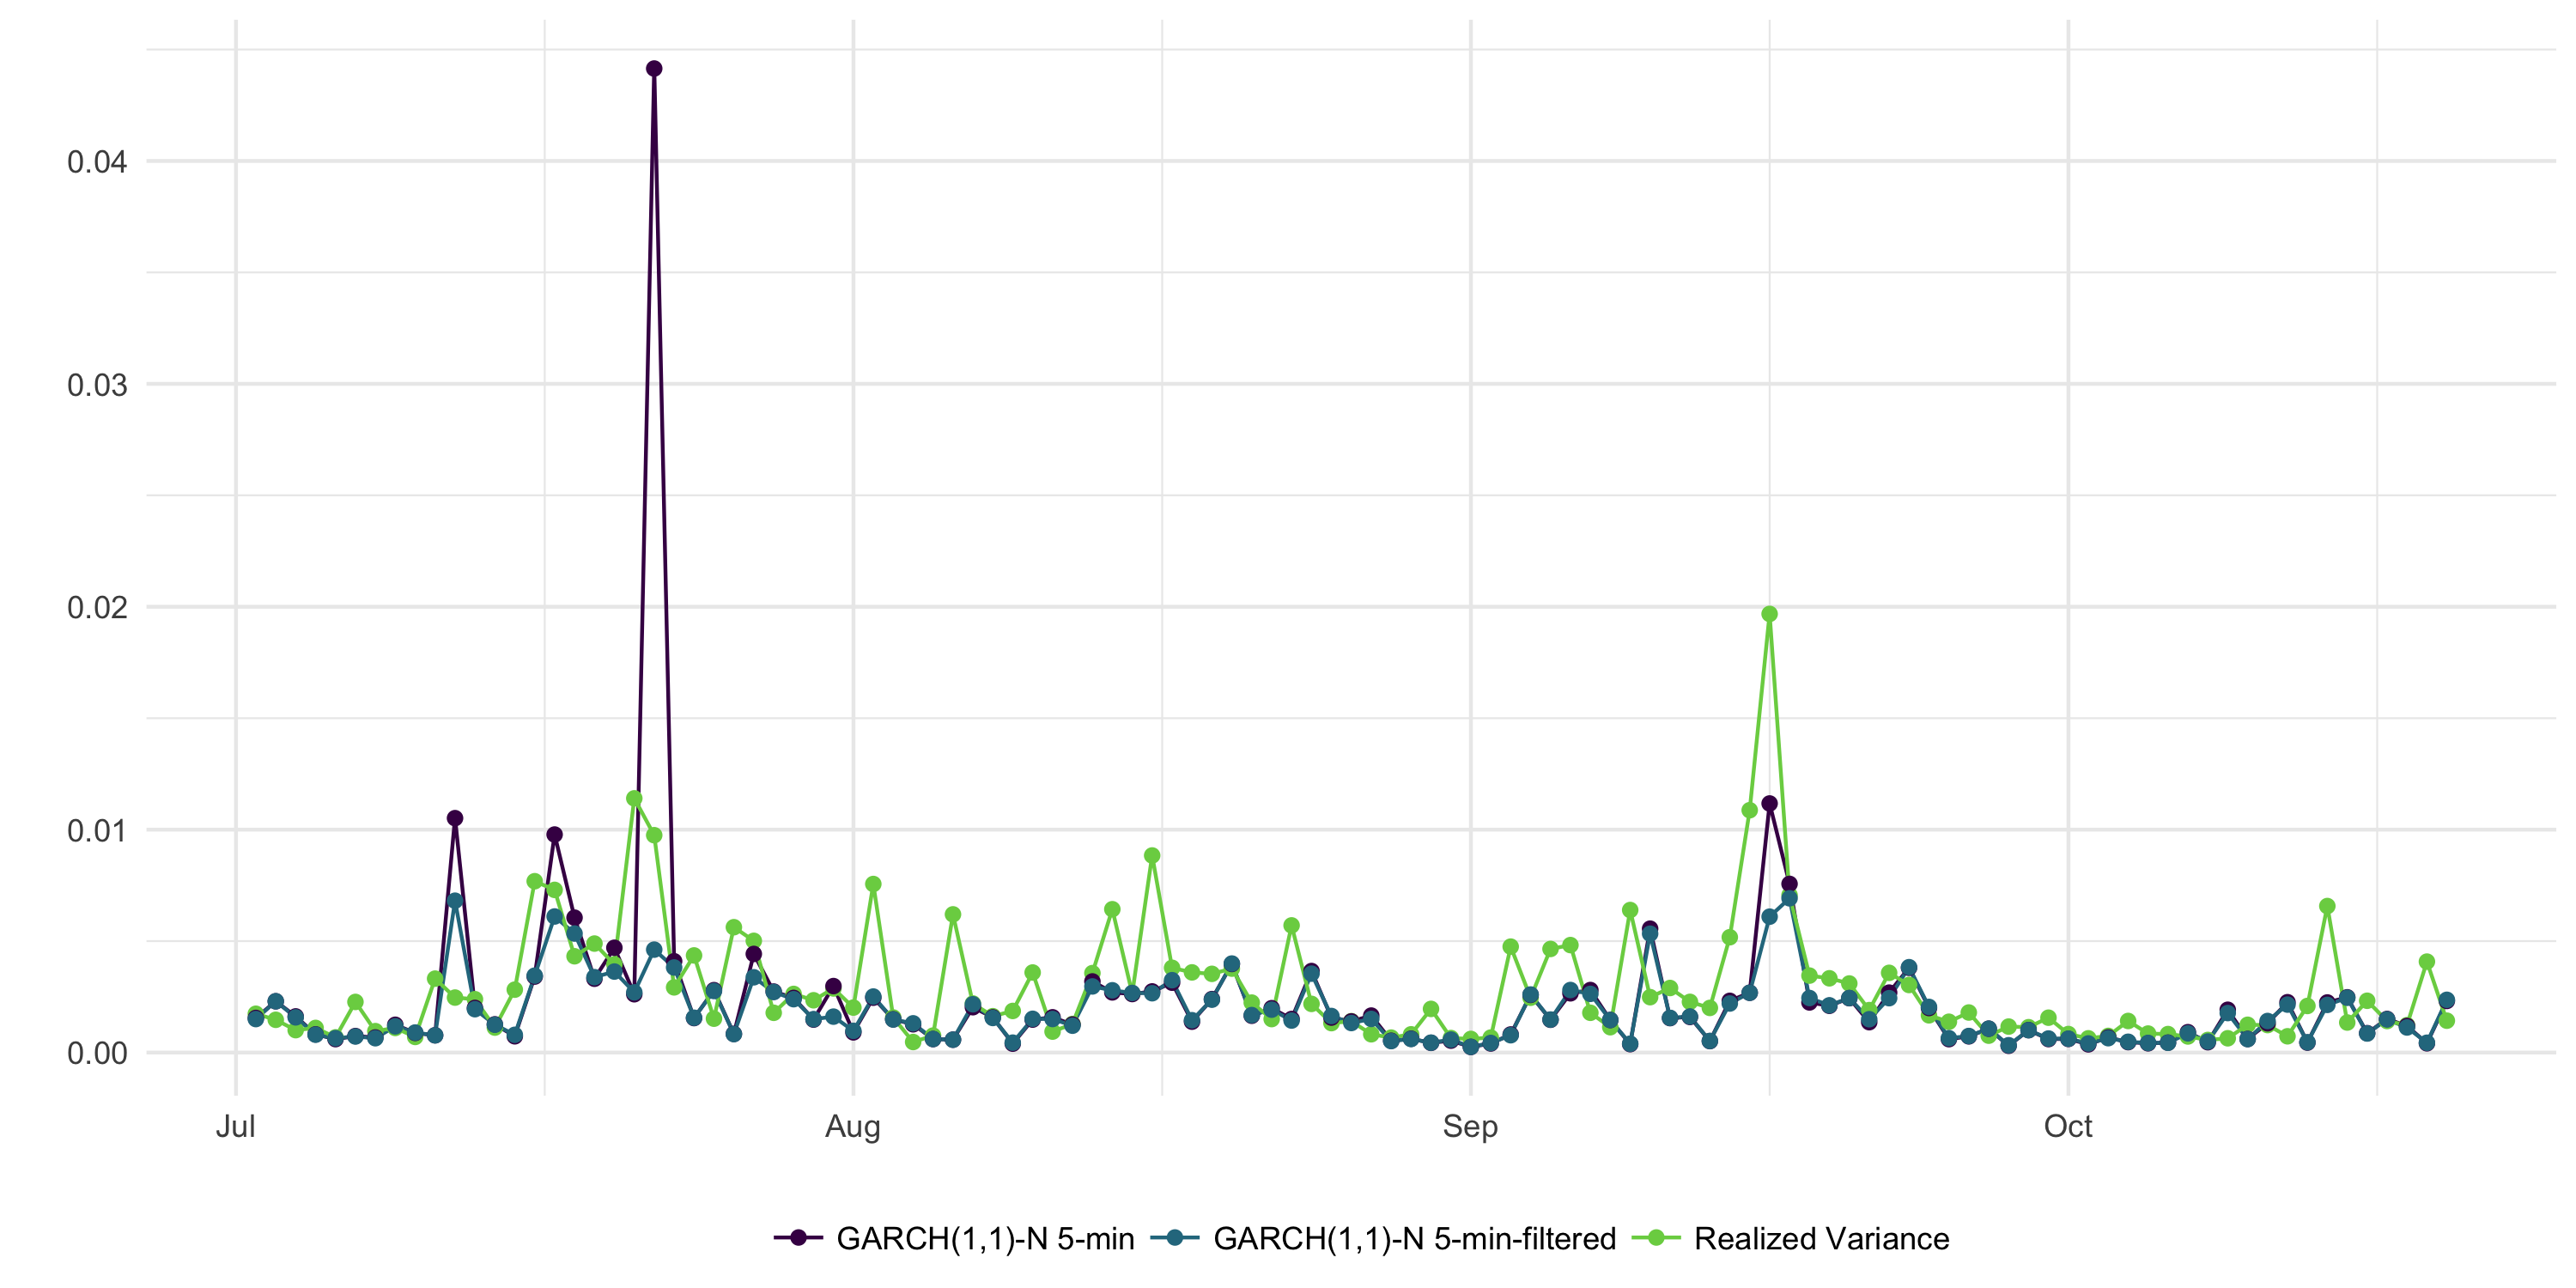
\includegraphics[width=1.00\textwidth]{../../visualizations/compare_normal_forecasts_filtered} 
  \end{center}
  \caption{Comparing filtered 5-minute variance forecasts with 5-minute variance forecasts. The filtration dampned the effects of the unusual 5-minute returns in July.}\label{fig}
\end{figure*}

\begin{table}[h]
\centering\captionsetup{justification=centering,singlelinecheck=off}
\caption{Forecast performance of the filtered 5-minute model. Performance metrics are on par with the results from removing the extreme outlier from the non-filtered model.}
\begin{tabularx}{0.5\textwidth}{p{0.25\textwidth} p{0.25\textwidth}}
\multicolumn{1}{!{\color[RGB]{0, 0, 0}\vrule width 0pt}r!{\color[RGB]{0, 0, 0}\vrule width 0.3pt}}{\hspace*{10pt}\rule{0pt}{\baselineskip+10pt}\raggedleft \textbf{}\rule[-10pt]{0pt}{10pt}\hspace*{10pt}} & 
\multicolumn{1}{c!{\color[RGB]{0, 0, 0}\vrule width 0pt}}{\hspace*{10pt}\rule{0pt}{\baselineskip+10pt}\centering \textbf{5-Min Filtered}\rule[-10pt]{0pt}{10pt}\hspace*{10pt}}\tabularnewline[-0.5pt]


\hhline{>{\arrayrulecolor[RGB]{0, 0, 0}\global\arrayrulewidth=0.3pt}->{\arrayrulecolor[RGB]{0, 0, 0}\global\arrayrulewidth=0.3pt}|>{\arrayrulecolor[RGB]{0, 0, 0}\global\arrayrulewidth=0.3pt}-}
\arrayrulecolor{black}
\multicolumn{1}{!{\color[RGB]{0, 0, 0}\vrule width 0pt}r!{\color[RGB]{0, 0, 0}\vrule width 0.3pt}}{\hspace*{10pt}\rule{0pt}{\baselineskip+10pt}\raggedleft \textbf{Proxy: RV}\rule[-10pt]{0pt}{10pt}\hspace*{10pt}} & 
\multicolumn{1}{c!{\color[RGB]{0, 0, 0}\vrule width 0pt}}{\hspace*{10pt}\rule{0pt}{\baselineskip+10pt}\centering \rule[-10pt]{0pt}{10pt}\hspace*{10pt}}\tabularnewline[-0.5pt]
\multicolumn{1}{!{\color[RGB]{0, 0, 0}\vrule width 0pt}r!{\color[RGB]{0, 0, 0}\vrule width 0.3pt}}{\hspace*{10pt}\rule{0pt}{\baselineskip+10pt}\raggedleft MAPE\rule[-10pt]{0pt}{10pt}\hspace*{10pt}} & 
\multicolumn{1}{c!{\color[RGB]{0, 0, 0}\vrule width 0pt}}{\hspace*{10pt}\rule{0pt}{\baselineskip+10pt}\centering 0.0244\rule[-10pt]{0pt}{10pt}\hspace*{10pt}}\tabularnewline[-0.5pt]
\multicolumn{1}{!{\color[RGB]{0, 0, 0}\vrule width 0pt}r!{\color[RGB]{0, 0, 0}\vrule width 0.3pt}}{\hspace*{10pt}\rule{0pt}{\baselineskip+10pt}\raggedleft RMSE\rule[-10pt]{0pt}{10pt}\hspace*{10pt}} & 
\multicolumn{1}{c!{\color[RGB]{0, 0, 0}\vrule width 0pt}}{\hspace*{10pt}\rule{0pt}{\baselineskip+10pt}\centering 0.0026\rule[-10pt]{0pt}{10pt}\hspace*{10pt}}\tabularnewline[-0.5pt]
\multicolumn{1}{!{\color[RGB]{0, 0, 0}\vrule width 0pt}r!{\color[RGB]{0, 0, 0}\vrule width 0.3pt}}{\hspace*{10pt}\rule{0pt}{\baselineskip+10pt}\raggedleft MZ Intercept\rule[-0pt]{0pt}{0pt}\hspace*{10pt}} & 
\multicolumn{1}{c!{\color[RGB]{0, 0, 0}\vrule width 0pt}}{\hspace*{10pt}\rule{0pt}{\baselineskip+10pt}\centering 0.0010\rule[-0pt]{0pt}{0pt}\hspace*{10pt}}\tabularnewline[-0.5pt]
\multicolumn{1}{!{\color[RGB]{0, 0, 0}\vrule width 0pt}r!{\color[RGB]{0, 0, 0}\vrule width 0.3pt}}{\hspace*{10pt}\rule{0pt}{\baselineskip+0pt}\raggedleft \rule[-10pt]{0pt}{10pt}\hspace*{10pt}} & 
\multicolumn{1}{c!{\color[RGB]{0, 0, 0}\vrule width 0pt}}{\hspace*{10pt}\rule{0pt}{\baselineskip+0pt}\centering (0.00037)\rule[-10pt]{0pt}{10pt}\hspace*{10pt}}\tabularnewline[-0.5pt]
\multicolumn{1}{!{\color[RGB]{0, 0, 0}\vrule width 0pt}r!{\color[RGB]{0, 0, 0}\vrule width 0.3pt}}{\hspace*{10pt}\rule{0pt}{\baselineskip+10pt}\raggedleft MZ Slope\rule[-0pt]{0pt}{0pt}\hspace*{10pt}} & 
\multicolumn{1}{c!{\color[RGB]{0, 0, 0}\vrule width 0pt}}{\hspace*{10pt}\rule{0pt}{\baselineskip+10pt}\centering 1.0567\rule[-0pt]{0pt}{0pt}\hspace*{10pt}}\tabularnewline[-0.5pt]
\multicolumn{1}{!{\color[RGB]{0, 0, 0}\vrule width 0pt}r!{\color[RGB]{0, 0, 0}\vrule width 0.3pt}}{\hspace*{10pt}\rule{0pt}{\baselineskip+0pt}\raggedleft \rule[-10pt]{0pt}{10pt}\hspace*{10pt}} & 
\multicolumn{1}{c!{\color[RGB]{0, 0, 0}\vrule width 0pt}}{\hspace*{10pt}\rule{0pt}{\baselineskip+0pt}\centering (0.15876)\rule[-10pt]{0pt}{10pt}\hspace*{10pt}}\tabularnewline[-0.5pt]
\multicolumn{1}{!{\color[RGB]{0, 0, 0}\vrule width 0pt}r!{\color[RGB]{0, 0, 0}\vrule width 0.3pt}}{\hspace*{10pt}\rule{0pt}{\baselineskip+10pt}\raggedleft MZ $R^2$\rule[-10pt]{0pt}{10pt}\hspace*{10pt}} & 
\multicolumn{1}{c!{\color[RGB]{0, 0, 0}\vrule width 0pt}}{\hspace*{10pt}\rule{0pt}{\baselineskip+10pt}\centering 0.2890\rule[-10pt]{0pt}{10pt}\hspace*{10pt}}\tabularnewline[-0.5pt]


\hhline{>{\arrayrulecolor[RGB]{0, 0, 0}\global\arrayrulewidth=0.3pt}->{\arrayrulecolor[RGB]{0, 0, 0}\global\arrayrulewidth=0.3pt}|>{\arrayrulecolor[RGB]{0, 0, 0}\global\arrayrulewidth=0.3pt}-}
\arrayrulecolor{black}
\multicolumn{1}{!{\color[RGB]{0, 0, 0}\vrule width 0pt}r!{\color[RGB]{0, 0, 0}\vrule width 0.3pt}}{\hspace*{10pt}\rule{0pt}{\baselineskip+10pt}\raggedleft \textbf{Proxy: $r^2$}\rule[-10pt]{0pt}{10pt}\hspace*{10pt}} & 
\multicolumn{1}{c!{\color[RGB]{0, 0, 0}\vrule width 0pt}}{\hspace*{10pt}\rule{0pt}{\baselineskip+10pt}\centering \rule[-10pt]{0pt}{10pt}\hspace*{10pt}}\tabularnewline[-0.5pt]
\multicolumn{1}{!{\color[RGB]{0, 0, 0}\vrule width 0pt}r!{\color[RGB]{0, 0, 0}\vrule width 0.3pt}}{\hspace*{10pt}\rule{0pt}{\baselineskip+10pt}\raggedleft MAPE\rule[-10pt]{0pt}{10pt}\hspace*{10pt}} & 
\multicolumn{1}{c!{\color[RGB]{0, 0, 0}\vrule width 0pt}}{\hspace*{10pt}\rule{0pt}{\baselineskip+10pt}\centering 0.2666\rule[-10pt]{0pt}{10pt}\hspace*{10pt}}\tabularnewline[-0.5pt]
\multicolumn{1}{!{\color[RGB]{0, 0, 0}\vrule width 0pt}r!{\color[RGB]{0, 0, 0}\vrule width 0.3pt}}{\hspace*{10pt}\rule{0pt}{\baselineskip+10pt}\raggedleft RMSE\rule[-10pt]{0pt}{10pt}\hspace*{10pt}} & 
\multicolumn{1}{c!{\color[RGB]{0, 0, 0}\vrule width 0pt}}{\hspace*{10pt}\rule{0pt}{\baselineskip+10pt}\centering 0.0069\rule[-10pt]{0pt}{10pt}\hspace*{10pt}}\tabularnewline[-0.5pt]
\multicolumn{1}{!{\color[RGB]{0, 0, 0}\vrule width 0pt}r!{\color[RGB]{0, 0, 0}\vrule width 0.3pt}}{\hspace*{10pt}\rule{0pt}{\baselineskip+10pt}\raggedleft MZ Intercept\rule[-0pt]{0pt}{0pt}\hspace*{10pt}} & 
\multicolumn{1}{c!{\color[RGB]{0, 0, 0}\vrule width 0pt}}{\hspace*{10pt}\rule{0pt}{\baselineskip+10pt}\centering 0.0013\rule[-0pt]{0pt}{0pt}\hspace*{10pt}}\tabularnewline[-0.5pt]
\multicolumn{1}{!{\color[RGB]{0, 0, 0}\vrule width 0pt}r!{\color[RGB]{0, 0, 0}\vrule width 0.3pt}}{\hspace*{10pt}\rule{0pt}{\baselineskip+0pt}\raggedleft \rule[-10pt]{0pt}{10pt}\hspace*{10pt}} & 
\multicolumn{1}{c!{\color[RGB]{0, 0, 0}\vrule width 0pt}}{\hspace*{10pt}\rule{0pt}{\baselineskip+0pt}\centering (0.00109)\rule[-10pt]{0pt}{10pt}\hspace*{10pt}}\tabularnewline[-0.5pt]
\multicolumn{1}{!{\color[RGB]{0, 0, 0}\vrule width 0pt}r!{\color[RGB]{0, 0, 0}\vrule width 0.3pt}}{\hspace*{10pt}\rule{0pt}{\baselineskip+10pt}\raggedleft MZ Slope\rule[-0pt]{0pt}{0pt}\hspace*{10pt}} & 
\multicolumn{1}{c!{\color[RGB]{0, 0, 0}\vrule width 0pt}}{\hspace*{10pt}\rule{0pt}{\baselineskip+10pt}\centering 0.8692\rule[-0pt]{0pt}{0pt}\hspace*{10pt}}\tabularnewline[-0.5pt]
\multicolumn{1}{!{\color[RGB]{0, 0, 0}\vrule width 0pt}r!{\color[RGB]{0, 0, 0}\vrule width 0.3pt}}{\hspace*{10pt}\rule{0pt}{\baselineskip+0pt}\raggedleft \rule[-10pt]{0pt}{10pt}\hspace*{10pt}} & 
\multicolumn{1}{c!{\color[RGB]{0, 0, 0}\vrule width 0pt}}{\hspace*{10pt}\rule{0pt}{\baselineskip+0pt}\centering (0.46461)\rule[-10pt]{0pt}{10pt}\hspace*{10pt}}\tabularnewline[-0.5pt]
\multicolumn{1}{!{\color[RGB]{0, 0, 0}\vrule width 0pt}r!{\color[RGB]{0, 0, 0}\vrule width 0.3pt}}{\hspace*{10pt}\rule{0pt}{\baselineskip+10pt}\raggedleft MZ $R^2$\rule[-10pt]{0pt}{10pt}\hspace*{10pt}} & 
\multicolumn{1}{c!{\color[RGB]{0, 0, 0}\vrule width 0pt}}{\hspace*{10pt}\rule{0pt}{\baselineskip+10pt}\centering 0.0311\rule[-10pt]{0pt}{10pt}\hspace*{10pt}}\tabularnewline[-0.5pt]
\end{tabularx}

\end{table}

\section{Conclusion}\label{conclusion}

This paper analyzed the daily volatility of Bitcoin returns using GARCH
modeling. Of note, two forecasting techniques were used, a traditional
forecasting method where the model is fit to daily data to predict daily
data, and a more granular model fit to 5-minute data where daily
forecasts are generated from aggregating multi-step ahead 5-minute
forecasts. The performance was measured against two proxies, the common,
but noisy, daily squared return, and realized variance.

Forecasts generated from the 5-minute method were overall more accurate
than traditional GARCH modeling forecasts, but care must be taken to
deal with outliers. Models fit under the Normal distribution do not
produce forecasts that are practically different from Student-t
distributions. The realized variance proxy is a much more promising
estimate of daily variance than the squared daily return. Looking only
at the MZ regression \(R^2\) values demonstrates this, where forecasts
compared against daily squared returns present \(R^2\) values near 0.

Future research could focus on creating models that better handled the
large swings in short term volatility so that a filtration would not
have to be applied. Additionally, other modeling periodicities could be
tried to find an optimal forecasting granularity.

%\showmatmethods
\showacknow


\bibliography{pinp}
\bibliographystyle{jss}



\end{document}

